\documentclass[12pt]{book}
\usepackage[colorlinks=true,linkcolor=blue,urlcolor=black]{hyperref}
\usepackage{bookmark}
\usepackage[margin=1in]{geometry}
\usepackage{graphicx}
\usepackage{float}

\title{\vspace{-1.5cm}Module 3- Network Systems Notes}
\author{Puru Vaish\\Department Of Technical Computer Science}
\date{\today}

\setlength{\parskip}{0.5em}

\begin{document}

\maketitle
\chapter{Chapter 1: Foundation}
\section{Applications}
\begin{enumerate}
    \item VOIP- Voice Over Internet Protocol
    \item Streaming
    \item HTML pages, i.e. Surfing the world wide web\\
    Downloading pages from the internet.
    \item Video Calls
\end{enumerate}
\section{Requirements of the Applications}
This section is about why are networks made the way they are, and not why they should be done in only one particular way. As time and needs progress the way networks work may change. 
\subsection{Shareholders}
First, we shall look at the requirements "from" a network from three different perspectives of shareholders.
\begin{enumerate}
    \item Application Programmer:
    the services that his or her application needs: for example, a guarantee that each message the application sends will be delivered without error within a certain amount of time or the ability to switch gracefully among different connections to the network as the user moves around.
    \item Network Operator (person who is in charge f debugging a network, configuring a network): These people in real life are likely IT managers in businesses who make sure the 'system network' is not crashing. Hence, they would want a network which is easy to isolate faults in, add/remove systems, account for usage (all the people who use streaming services can be listed).
    \item Network designer: Efficiency, usability, performance are the key topics here.
\end{enumerate}

\subsection{Scalability}
Networks in general should be scalable, i.e. it should be possible to add more nodes to the network without affecting the network, for example, having to close down the network temporarily, or even without a drop of performance, and not effecting other users while removal or addition.
\begin{enumerate}
    \item BAD:
    \begin{enumerate}
        \item Bus Networks- Too usch stress on the main line, when more users are added
        \item Ring- Can not add more users without disturbing other users, or taking down the system, unnecesary traffic onto adjacent connections.
        \item Mesh- Too many connections, tht are likely not being used, too much cabling required, not possible to connect 1000 nodes like this, simply not enough ports if you think about it.
    \end{enumerate}
    \item GOOD:
    \begin{enumerate}
        \item Star- at least as a component.
        \item P2P- not without it's own problems.
    \end{enumerate}
\end{enumerate}
Notice in the GOOD section, we have network topologies that do have some problems as well, but are more easily scaled than the previous ones.

General Note: Two nodes need not have a direct link between them, but even an indirect link through several nodes. In such a scenario it is easy to see how using existing connections in start network or P2P, outweigh something like Mesh, or Bus. 

\subsection{Cost Effective Resource Sharing}
Hosts on a network have to share its resources, the resource we are most interested in is the data transmission medium (usually a copper cable, optic fibre or radio waves), this sharing is called multiplexing, which means that a system resource is shared among multiple users. At an intuitive level, multiplexing can be explained by analogy to a timesharing computer system, where a single physical processor is shared (multiplexed) among multiple jobs, each of which believes it has its own private processor. Similarly, data being sent by multiple users can be multiplexed over the physical links that make up a network.

There are different ways of sharing resources under two different schemes:
\begin{enumerate}
    \item Circuit Switching
    \begin{enumerate}
        \item What happens in this scheme:
        \begin{enumerate}
            \item One node pings the destination node, possibly using some hello message.
            \item If no response, waits, else proceeds to establish a connection according to the protocol AND (MORE IMP) fixes a route between the two nodes by fixing hops between the routers of the two nodes. (Since this path is fixed it can NOT be shared by other users of the network).
            \item The users transmit data along this dedicated route.
            \item packet receival is guaranteed unless a calamity happens (routers between hops gets disconnected, or the users themselves are disconnected).
            \item the connection is torn down, once 'bye' is done.
        \end{enumerate}
        \item Why Bad?\\
            In reality, the two computers may not be communicating all the time. So, say they are connected, and so the router had to fix this route which takes 25\% of the bandwidth of the path. If they do not communicate this is all wasted.\\
            The way the resource is allocated in this scheme are:
            \begin{enumerate}
                \item STDM: Synchronous Time Disvision multiplexing.\\
                The name is self explanatory, according to the number of users who use the link, it divides the time axis by the number of connections and then sends the data over those time periods. This is similar to Round-Robin approach where each connection between the nodes needs to wait it's turn.
                \item FDM: Frequency Division Multiplexing.\\
                The name is again self explanatory. Instead of diving the time axis, the frequency axis is divided (think of radio waves of different frequencies). Each connection is then given a frequency through which the data is then sent which is distinct from the other frequencies (so that they do not interfere in terms of data being carried) and then the data is then delivered.
            \end{enumerate}
            \item Nether of schemes solve the problem of the fact the path is held busy even when there are no transmissions and hence leads to an upper bound of the number of connections the connection can handle before people have to start waiting for their turn. For example: if each connection 'requires' (application requirement alert) to send at a speed of 1Mbps on a 10Mbps link but only transmits at a probability of 10\% the connection can handle at best 10 nodes at the same time due to the link capacity, otherwise it may have to drop packets, store them, etc.
    \end{enumerate}
    \item Packet Switching
    \begin{enumerate}
        \item What happens in this scheme (Also the description of statistical multiplexing):
        \begin{enumerate}
            \item The packet is prepared by the computer system.
            \item The packet route is then simply resolved, which means the path it needs to take to the destination is determined.
            \item each packet can take a different route.
            \item It then reaches the destination after getting routed by each router.
            \item If the destination is unavailable, that is okay, it can try again, else the message id delivered, and the destination computer takes care of all the packets arriving.
            \item notice, the route taken is never fixed, and never kept busy for this particular connections.
        \end{enumerate}
        \item Why Good?\\
        It allows sharing of resources. Consider the above example again, this time 35 users can access the same system the entire time, since the probability that more than 10 users are active at the same time is actually less than 0.004. Allowing more efficient data bandwidth usage, as it supports greater variety of connections. (Notice: we do not say greater number of maximum connections, as that is still 10, but in circuit switching only 10 different permutations of connections are possible in a given time frame, while in packet switching 35 choose 10 connections are possible in a time frame (not instantaneously) as the connection is blocked for the first 10 only).\\\\
        Statistical Multiplexing is similar to STDM, only the time slots are not predefined, but on-demand. Also it determines who to transmit from similarly to STDM in a round-robin manner, such allocation of bandwidth is used to call such networks having Quality of Service (QoS).
    \end{enumerate}
\end{enumerate}

Even in switching there are two types on hardware level:
\begin{enumerate}
    \item Store-and-Forward: Store-and-Forward switchingwill wait until the entire frame has arrived prior to forwardingit. This method stores the entire frame in memory. Once the frameis in memory, the switch checks the destination address, sourceaddress, and the CRC. If no errors are present, the frame isforwarded to the appropriate port. This process ensures that thedestination network is not affected by corrupted or truncatedframes.
    \item Cut-Through: Cut-Through switching will beginforwarding the frame as soon as the destination address isidentified. The difference between this and Store-and-Forward isthat Store-and-Forward receives the whole frame before forwarding.Since frame errors cannot be detected by reading only thedestination address, Cut-Through may impact network performance byforwarding corrupted or truncated frames. These bad frames cancreate broadcast storms wherein several devices on the networkrespond to the corrupted frames simultaneously.
\end{enumerate}

The network obviously needs to ensure the proper packetisation of data, to ensure just one connections hogs the entire bandwidth and the rest of the connections end up getting nothing.

This does not mean that Circuit Switching is useless though, in some instances it may be more essential to have a dedicated connection rather than efficiency of resource sharing, but then networks likely need to be catered for such applications.

\subsection{Support for Common Services}
Think of WhatsApp, Messenger, Viber(?). They are all text messaging applications, or at least have that as one of their functions. The network needs to ensure that one instance of any of those application can communicate with another instance of the application. THis could be implmented all in the application itself, from protocol to creation of bits, but if they are all going to be doing the same tasks, (ask for authentication, generate bits using the same scheme, have IP addresses and so on) it makes sense to put it rather in the network implmentation. This is where layering comes in. The challenge is to find those abstractions which allow the greatest range of applications to be implemented, without constraining the Application Developer (If they had ocntrol of all parts they could do anything they wanted, the fact you take things away from their control may restrict them).\\
For example, does the application require a guarantee that messages sent over the channel are delivered, or is it acceptable if some messages fail to arrive? Is it necessary that messages arrive at the recipient process in the same order in which they are sent, or does the recipient not care about the order in which messages arrive? Does the network need to ensure that no third parties are able to eavesdrop on the channel, or is privacy not a concern? In general, a network provides a variety of different types of channels, with each application selecting the type that best meets its needs. The rest of this section illustrates the thinking involved in defining useful channels.

\subsection{Identify Common Communication Patterns}
How different are two applications. FTP/NFS they both transfer files but just in different ways, the entire file or in blocks. The underlying technology of sending the file (data) is not different. The network need to be concerned with the specifics but only the similarity.

\subsection{Reliable Message Delivery}
The causes why the message may not be delivered as sent/requested (apart from hacker activity)
\begin{enumerate}
    \item Packet may switch bits over the link: noise, radiation. How can flip the bit maybe? Does it need to be discarded.
    \item Packet itself may not arrive: queue, dropped. How to determine packet is lost and not just late? Sent to wrong connection.
    \item The node and link layer may lose connection: Power Outage, mis-configuration of the network, reckless operator.
\end{enumerate}

\subsection{Manageability}
Network system need to be manageable. This includes:
\begin{enumerate}
    \item How to keep track of addresses?
    \item Track of usages?
    \item Troubleshoot in case of problems
    \item Change to new equipment, add functionality.
\end{enumerate}

A general ideology is used to keep away when it works, which promotes a slow progress in features available as stability is more focused upon.

\section{Architecture}
\subsection{Layering and Protocols}
Layering provides two benefits:
\begin{enumerate}
    \item First, it decomposes the problem of building a network into more manageable components. Rather than implementing a monolithic piece of software that does everything you will ever want, you can implement several layers, each of which solves one part of the problem. 
    \item Second, it provides a more modular design. If you decide that you want to add some new service, you may only need to modify the functionality at one layer, reusing the functions provided at all the other layers.
\end{enumerate}

Layering allows for different methods of communication. For example:
\begin{enumerate}
    \item Request/Reply Protocol
    \item Message Stream Protocol
\end{enumerate}
Why? Because protocol is nothing but abstracted objects that make up the layers, which tell the higher layers how the data is to be handled, how the data was formatted, and not what the actual data is. But, how is it seen computationally by a a device? Each protocol defines two different interfaces:

\begin{enumerate}
    \item First, it defines a service interface to the other objects on the same computer that want to use its communication services. This service interface defines the operations that local objects can perform on the protocol. For example, a request/reply protocol would support operations by which an application can send and receive messages. An implementation of the HTTP protocol could support an operation to fetch a page of hypertext from a remote server. An application such as a web browser would invoke such an operation whenever the browser needs to obtain a new page (e.g., when the user clicks on a link in the currently displayed page).
    \item Second, a protocol defines a peer interface to its counterpart (peer) on another machine. This second interface defines the form and meaning of messages exchanged between protocol peers to implement the communication service. This would determine the way in which a request/reply protocol on one machine communicates with its peer on another machine. In the case of HTTP, for example, the protocol specification defines in detail how a GET command is formatted, what arguments can be used with the command, and how a web server should respond when it receives such a command.
\end{enumerate}

But these details are not important, what is important is to understand that in either of these two methods of sending data, they are not any different for lower protocols, only on higher protocol on both receiving and sending side. Diving up the stack in these abstract entities allows other protocols like HHP (Host to Host protocol) which acquires connection for the hosts, or SIP (Session initiation Protocol) which acquires the knowledge of the contacted peer, Geographic, capability, availability, session setup and session management to be achieved.

To further understand how layering is actually implemented despite so many protocols, we look at encapsulation.

\subsection{Encapsulation}
The only thing to get in this subsubsection is what are headers. Application Layer collects data to be sent. Transport Layer packetises everything and adds a header $\to$ giving each packet a dest. and src. port packet number, checksum and relevant data in the header. The network protocol adds IP addresses, tolive, IP version, frgamentation limit and so on it its header, and so on for each protocol that is encountered. This adding of headers upon headers is the essence and what encapsulation is. The peer need not read the entire thing, strip of the header and pass along if the packet is of the node on the network.

\subsection{Multiplexing and Demultiplexing}
Since we are considering archtecture it is appropriate to think about how a network handles Multiplexing and Demultiplexing. Simple: Using keys. Each application would generate jeys, or even multiple keys either specific for that connection or some other arbitrary way and pass that along in the protocol being used (RRP or MSP), according to the application's implementation of the protocol (as applications care only about intra application communication, yes there is PC XBOX cross-platform gaming but those are special cases where they may use some sort of translators) and then communicate. These are called demux keys.

\subsection{Internet Architecture}

(We will not discuss the 5 layers of internet here:
Application, Transport, Network, Link, Physical. These are talked about all the time anyway.)

Since internet is a part of the network, we shall give a brief of description of that as well. Internet as we know and use, has three different attributes:
\begin{enumerate}
    \item First, as best illustrated by Figure 15, the Internet architecture does not imply strict layering. The application is free to bypass the defined transport layers and to directly use IP or one of the underlying networks. In fact, programmers are free to define new channel abstractions or applications that run on top of any of the existing protocols.
    
    \item Second, if you look closely at the protocol graph in Figure 14, you will notice an hourglass shape—wide at the top, narrow in the middle, and wide at the bottom. This shape actually reflects the central philosophy of the architecture. That is, IP serves as the focal point for the architecture—it defines a common method for exchanging packets among a wide collection of networks. Above IP there can be arbitrarily many transport protocols, each offering a different channel abstraction to application programs. Thus, the issue of delivering messages from host to host is completely separated from the issue of providing a useful process-to-process communication service. Below IP, the architecture allows for arbitrarily many different network technologies, ranging from Ethernet to wireless to single point-to-point links.
    \item A final attribute of the Internet architecture (or more accurately, of the IETF culture) is that in order for a new protocol to be officially included in the architecture, there must be both a protocol specification and at least one (and preferably two) representative implementations of the specification. The existence of working implementations is required for standards to be adopted by the IETF. This cultural assumption of the design community helps to ensure that the architecture’s protocols can be efficiently implemented.
\end{enumerate}

\section{Software}
\section{Performance}
Time for some calculation now.
\subsection{Bandwidth and Latency}
What is quick?
\begin{enumerate}
    \item I can get big files quick- High Bandwidth (throughput)\\
    Depended on:
    \begin{enumerate}
        \item Size of the 'pipes' we use to send data.\\
        This is basically the transmission rate of the cable.
    \end{enumerate}
    \item I can get a response quickly- Low Latency (delay)\\
    Depended on:
    \begin{enumerate}
        \item The physical distance between two points
        \item the length of cabling
        \item the transmission method being used.\\
        (All these things effectively correspond to the RTT (Round Trip Time))
    \end{enumerate}
\end{enumerate}
Note: RTT not same as 2 x One way trip, we will see why. Although in many instances it can give a good approximation.

\subsection{DBP- Delay Bandwidth Product}
(Personal Note- In middle school we had this question which revolved around thinking of time as a length and the rate of flow as the width, so their product gave us the volume. If we talk about the units $m^{3}s^{-1} * s = m^{3}$, i.e. the volume)

Using my personal note, I hope it is clear then why I say this Delay Bandwidth Product is actually the number of bits this pipe is carrying (amount of water in the pipe). The bandwidth is the flow rate, and the delay is the time the bits stay in the pipe for, hence you can not add more bits to the pipe in that frame since we are travelling at the max flow rate. Using this analogy we understand why the delay product is a good measure of performance.//
This should not be confused with the DBP giving an indication on how good a particular network is in only one of the metrics. High BDP could simply mean a very high delay time, similarly a low DBP could mean a very low delay time. This serves kind of like a general view on how good something is, overall.

Let us look at some examples:
\subsection{Q1}
Handshake = 0.1s
B = 1.5MBps
L = 1000Kb
RTT = 50ms
Packet Size = 1Kb

Find total delay if sent continuously.
\begin{enumerate}
    \item One Pipe    = B*(RTT/2) 37500bits
    \item number      = L/One Pipe 218.45333 pipes
    \item total Time  = number*(RTT/2) 218.4533*25ms = 5.46133s
    \item add         = handshake time 0.1s
    \item add the length of the last pipe, since the length is time 25ms
    \item total delay = 5.586s
\end{enumerate}
(Note we talking about bits, do not forget to convert from bytes to bits)
\subsection{Q2}
after every packet is sent we will wait for 1RTT.
this is where we must understand the distinction between different delays, namely, Transmission Delay and Propagation delay.
\begin{enumerate}
    \item how long does it take to transmit a packet: 1kb/B
    \item how long does it take for the packet to propogate: RTT/2
    \item how long do we wait: 1RTT
    \item but since in the same time the packet has travelled to the other side we can say the RTT/2 is contained in the 1RTT.
\end{enumerate}
Calc:
\begin{enumerate}
    \item handshake = 0.1s
    \item one packet sent = RTT + TD
    \item 1000packets sent = 1000*one packet - RTT (since we do not wait for last packet ack)
    \item pipe length = 0.025s (we need this even if only one bit is sent)
    \item total = 55.536s
\end{enumerate}

(No shortcut please, add everything slowly slowly).

\subsection{Throughput calculations.}

Throughput = TransferSize / TransferTime \\
TransferTime = RTT + TransferSize/Bandwidth\par

These ones can be a bit weird depending on the answer, you may not see why they chose to ignore some bits.\par
Q3) 12000bit packets are sent only after getting a 50byte ack from receiver on a link with three switches which add 10us for every pass and the link itself has a B of 100MBps.
\begin{enumerate}
    \item transmission rate = 12000/100*$10^{6}$ = 120us
    \item there are three switches so total 4 times on switch then on link (draw, please): 4*120us = 480us
    \item each switch adds 10us, but don't forget on receiver we have to read too so +40us = 520us.
    \item next packet not sent until 50byte ack is received. each transmission of ack takes 50*8/100*$10^{6}$ = 4us. Notice, this is done 4 times, and also it follows the same 10us 4 times thing since it goes through the same switches. So, +4*(10 + 4) = 56us
    \item total = 576us.
    \item Now how much data actually transferred = 12000bits (why not +50 bytes, cause that is ack).
    \item How much time taken = 576us.
    \item So actual throughput = 12000bits/576us = 20.833Mbps.
\end{enumerate}
(this is an okay question once you know what is happening, you need to have an image in your head, and see all components work, links switches end receiver. the question itself is never clear sadly).\par
(no propagation delay specified for this question, but feel free to add that every time a packet travels over the Ethernet, which makes throughput even less.)\parskip\parskip

One last thing to consider is there may be times when transmission times are actually so low, that RTT ends up determining the delay entirely (especially when very high transmission cables are used).

\chapter{Chapter 2: Direct Links}

\section{Encoding}

Things we are worried about.
\begin{enumerate}
    \item baseline wander: he receiver keeps an average of the signal it has seen so far and then uses this average to distinguish between low and high signals. Whenever the signal is significantly lower than this average, the receiver concludes that it has just seen a 0; likewise, a signal that is significantly higher than the average is interpreted to be a 1. The problem, of course, is that too many consecutive 1s or 0s cause this average to change, making it more difficult to detect a significant change in the signal.
    \item clock recovery: The receiver derives the clock from the received signal—the clock recovery process. Whenever the signal changes, such as on a transition from 1 to 0 or from 0 to 1, then the receiver knows it is at a clock cycle boundary, and it can re-synchronize itself. However, a long period of time without such a transition leads to clock drift.
\end{enumerate}

\subsection{NRZ}
Non-Return to Zero: basically high is 1, low is zero, nothing special. Solves nothing: long length of 0/1 possible.

\subsection{NRZI}
non-return to zero inverted: toggle if 1 on the clock, and if 0 then just there. Solves long length of 1's. Problem: what if long length of zeroes. (Solved using 4B/5B).

\subsection{Manchester}
Clock XOR NRZ data.\\
It doubles the transition rate of 1 $\to$ 0 and 0 $\to$ 1. The rate of transition is called baud rate. The bit rate is half of this. So in essence, the efficiency is half since the receiver is working twice the amount to get half the data. (This is the case only if you have 2 "symbols" high and low. Having more allows more data to be transmitted, which allows bit rate to be even higher than baud rate, so efficiency is 2x or more. Look up QAM).

\subsection{4B/5B and 8B/10B}
Use 5 bits to represent a data of 4 bits, and 10 for 8. The mapping is used to eliminate the long lengths of 0's and 1's which result in baseline wander. Three consecutive zero bits only appear in normal data when a code ending with two 0 bits (2, E) is followed by a code beginning with a 0 bit (1, 4, 5, 6), so will always appear separated by multiples of the 5-bit encoded symbol length (and never separated by a single symbol) i.e. no code has more than 2 zero at the start and more than 1 zero at beginning. Then transmit using NRZI. Since only 1 extra bit sent, the efficiency is 80\%.

\section{Framing}
How to know the bits collected by the adapter form a complete frame? Remember, the networks communicate with frames not series of bits.
\subsection{Byte Oriented Protocol}
Recent example of this is Point-to-Point Protocol (PPP). Two approaches to implement this.
\begin{enumerate}
    \item Sentinel Characters: STX, ACK, ETX stuff like this are put for beginning of frame, ending of frame. What if they appear in text. We use Data Link Escape (DLE) character. In \LaTeX we preceed comment or mathematical operator using backslash to ensure not to go to math mode \^, \%. Called character stufing.
    \item Include Count of number of bits, size of frame in the header. One danger with this approach is that a transmission error could corrupt the count field, in which case the end of the frame would not be correctly detected, leading to a framing error (more or less bytes accumulated).
\end{enumerate}
The internet protocol uses Sentinel Characters with character stuffing. The PPP frame is negotiated using Link Control Protocol (LCP) which is a frame itself sent over in PPP frame.

\subsection{Bit Oriented Protocol}
The Synchronous Data Link Control (SDLC) protocol developed by IBM is an example of a bit-oriented protocol; SDLC was later standardized by the ISO as the High-Level Data Link Control (HDLC) protocol.\\

HDLC denotes both the beginning and the end of a frame with the distinguished bit sequence 01111110. This sequence is also transmitted during any times that the link is idle so that the sender and receiver can keep their clocks synchronized. Because this sequence might appear anywhere in the body of the frame—in fact, the bits 01111110 might cross byte boundaries—bit-oriented protocols use the analog of the DLE character, a technique known as bit stuffing: \begin{enumerate}
    \item 011111 is seen in text.
    \item add 0: 01111100 $\to$ is the bit stuffing
    \item on receivers side, when 5 bits are seen, check next bit. if 1 then end of frame, if 0 then stuffing so remove this, if 1 and next is also 1: 01111111: this is error so discard frame.
\end{enumerate}

Both Bit/Byte Oriented Protocol have variable frame length due to their being stuffing. Next one is not variable length.

\subsection{Clock Based Framing}
A third approach to framing is exemplified by the Synchronous Optical Network (SONET) standard. SONET is very bid and can be covered in a book of itself. Also, SONET addresses both the framing problem and the encoding problem. It also addresses a problem that is very important for phone companies—the multiplexing of several low-speed links onto one high-speed link. (In fact, much of SONET’s design reflects the fact that phone companies have to be concerned with multiplexing large numbers of the 64-kbps channels that traditionally are used for telephone calls).

read implementation from the book.
Key Points:
\begin{enumerate}
    \item Easy to synchronize,
    \item allows multiple data rate, for each a different sized frame, better reception
    \item N STS-1 make up STS-Nc frame where c stands for concatenated, done by interleaving N STS-1 frames to create a bigger frame if link allows. So precisely- STS Nc is N*STS-1 frames, it is quantized.
    \item has overhead, and points to starting of the other, so in case frames are shifted for whatever reason, the receiver can resynchronize.
\end{enumerate}

\begin{figure}[H]
    \centering
    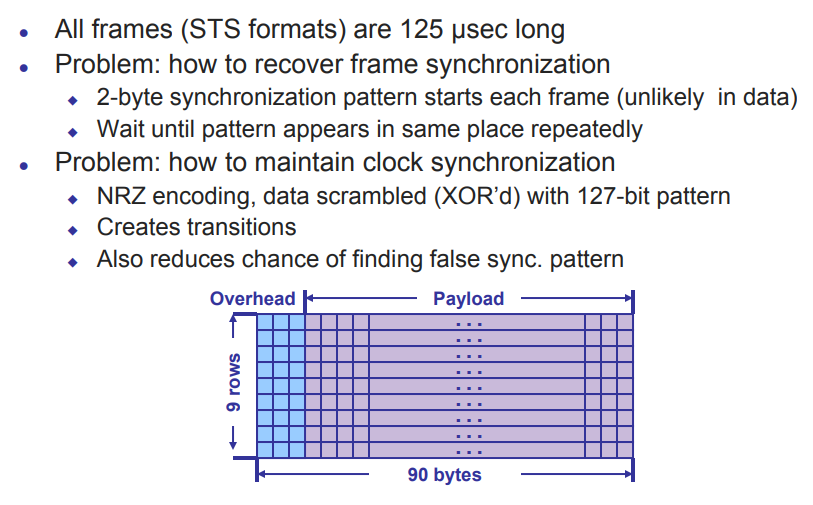
\includegraphics[width = \textwidth]{Pictures/SONET1.png}
    \caption{Caption}
    \label{fig:my_label}
\end{figure}
\begin{figure}[H]
    \centering
    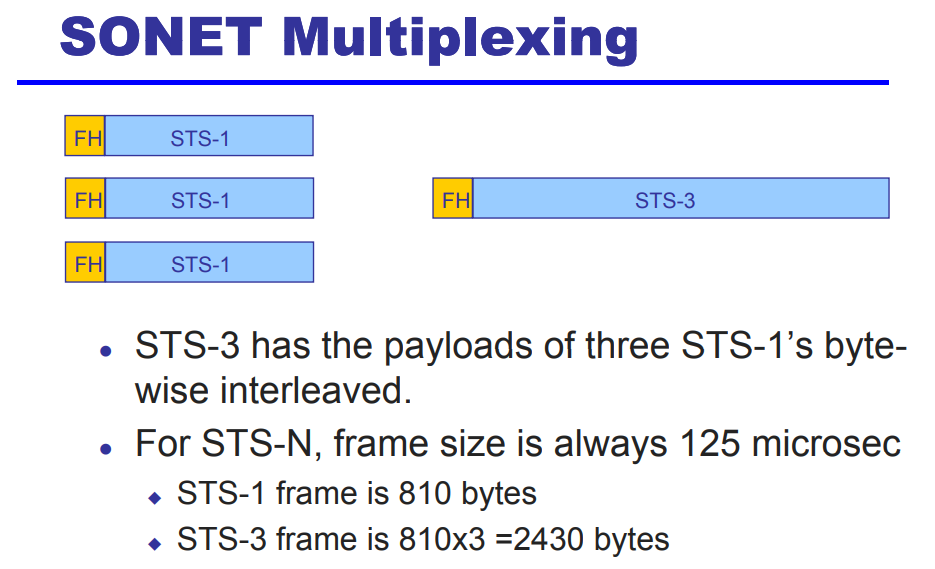
\includegraphics[width = \textwidth]{Pictures/SONET2.png}
    \caption{Caption}
    \label{fig:my_label}
\end{figure}
\begin{figure}[H]
    \centering
    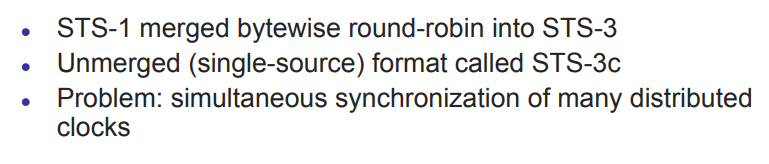
\includegraphics[width = \textwidth]{Pictures/SONET3.png}
    \label{fig:my_label}
\end{figure}
\begin{figure}[H]
    \centering
    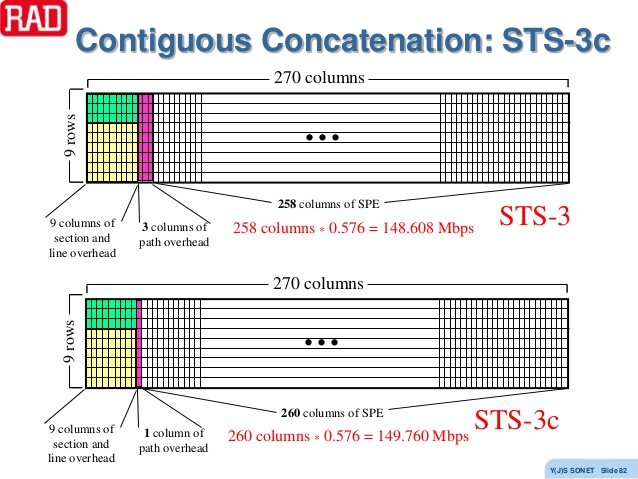
\includegraphics[width = \textwidth]{Pictures/sonet STS 3c vs STS 3.jpg}
    \caption{Caption}
    \label{fig:my_label}
\end{figure}

\section{Error Detection}
\subsection{Checksum}
Sum up the messages, discard overhead, transmit with block. Nothing to write about. This is a simple error detection technique, which is not even the most efficient.
\subsection{Parity Check}
Look up in the reader. Should be familiar with the process of doing this, nothing to write about. Look up in the reader.
\subsection{CRC- Circular Redundancy Check}
The polynomial arithmetic, long division, XOR-ing. Look up in th reader. Process summarized below.
\begin{enumerate}
    \item M(x) = message polynomial
    \item C(X) = generated polynomial, look up in reference, not calculated
    \item R(x) = calculated using the two above, M(x)*$x^{r}$ where r is the order of the polynomial of C(x), the calculation is then M(X)*$x^{r}$/C(x) = R(X), this is the long division step done using XOR operation.
    \item P(x) = polynomial to send = M(x) XOR R(x).
    \item guarantees remainder is zero when divided by the polynomial C(x) as we just subtracted the remainder(when we XOR that is what happens since we are using modulo 2 arithmetic).
    \item send
    \item recalculate $\to$ if not remainder 0, then problem.
\end{enumerate}
\subsection{Shannon's Mathematical Theory of Communication}
Only main topics are noted, most of this is intuition based and all formulae, nothing to write, other than reminding that these topics exist.
\begin{enumerate}
    \item Channel Capacity
    \item Amount of information in data - Huffman Coding
    \item Entropy
    \item Average number of bits.
    \item Error Detection vs Error Correction (i.e. which has more overhead).
    \item Entropy of a message * number of messages/s = information in message * messages/s = avg. no of bits per message * messages / s = avg number of bits / s.
\end{enumerate}
\section{Reliable Transmission}
Two things to be concerned about:
Reliable delivery is usually accomplished using a combination of two fundamental mechanisms—acknowledgments and timeouts. An acknowledgment (ACK for short) is a small control frame that a protocol sends back to its peer saying that it has received an earlier frame. By control frame we mean a header without any data, although a protocol can piggyback an ACK on a data frame it just happens to be sending in the opposite direction. The receipt of an acknowledgment indicates to the sender of the original frame that its frame was successfully delivered. If the sender does not receive an acknowledgment after a reasonable amount of time, then it retransmits the original frame. This action of waiting a reasonable amount of time is called a timeout.
\begin{enumerate}
    \item Acknowledgements= Did you receive what I sent?
    \item Timeout= Is it time for me to resend what I sent?
\end{enumerate}
Rest of the section discusses the algorithms for ack/timeout.

\begin{enumerate}
    \item Alternating Bit protocol
    \item Stop-Wait
    \item Sliding Window (please be familiar with all the acronyms- LAR, LFS, SWS -- LAS, LAF, RWS)
\end{enumerate}

\section{Multi-Access Networks}
\subsection{Physical Properties of Ethernet}
\begin{enumerate}
    \item CSMA\textbackslash CD Carrier Sense Multi Access, Collision Detection
    \item Repeaters
    \item length-maximal 2500m
    \item single length is only 500m, so up to 4 repeaters max.
\end{enumerate}

\subsection{Access Protocol}
\begin{enumerate}
    \item Frame Format:
    \begin{enumerate}
        \item Premeable- 64bits: to synchronize the signal. Similar to how SONET was described.
        \item Addresses- 48bits each Dest, Src.
        \item Type- Demux key, used for seeing if needs to be passed to higher protocol.
        \item Body
        \item CRC- 32bit
    \end{enumerate}
    \item Addresses:
    \begin{enumerate}
        \item MAC address. e.g. 8:0:2b:e4:b1:2.
    \end{enumerate}
\end{enumerate}

\subsection{Transmitter Algorithm}
\begin{enumerate}
    \item if idle send. Maximal length of frame = 1500 bytes (for fairness).
    \item if busy, calc random time, wait random time, try again. Uses Exponential Backoff.
    \item At the moment an adaptor detects that its frame is colliding with another, it first makes sure to transmit a 32-bit jamming sequence and then stops the transmission. Thus, a transmitter will minimally send 96 bits in the case of a collision: 64-bit preamble plus 32-bit jamming sequence.
    \item Typically Ethernet for given setting has a minimum of 512 bits frame. This allows for a collision to be detected, otherwise the computer may go away and not know that a collision happened, as illustrated below. Use padding as required.
    \begin{figure}[H]
        \centering
        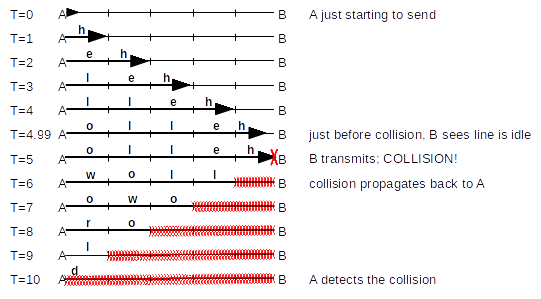
\includegraphics[width = \textwidth]{Pictures/MultiAccess- Collision Detection.png}
        \caption{Caption}
        \label{fig:my_label}
    \end{figure}
\end{enumerate}

\section{Wireless Networks}
\subsection{Medium}
read from reader, and slide mostly.

\subsection{Spread Spectrum}
\begin{enumerate}
    \item Frequency Hopping: Using a pseudorandom number generator (prng), jump to different frequency. The reciever has the same algorithm for the prng and so can follow the signal. Originally, Wifi typically uses 79- 1 MHZ bandwidth signals to jump across, all in 2.4GHz range.
    \item Direct Sequence Spread Spectrum: use a prng to create a chipping code. Use this code to encode the data to send. Originally, Wifi typically uses 11 bit chip code. If reciever does not have the same prng, the recieval is seen as random. This is called scrambling. Typically 1 bit is encoded to a length of 4, and then chip code is used to encode these 4 repated bits. Having more bits also increases tolerance to interference.
\end{enumerate}

\subsection{Different Methods of making connection}
\begin{enumerate}
    \item Base Station: Router, nodes can not communicate directly. The base station as it were, has no mobility, it meant to stay fixed. All communication occurs through it.
    \begin{figure}[H]
        \centering
        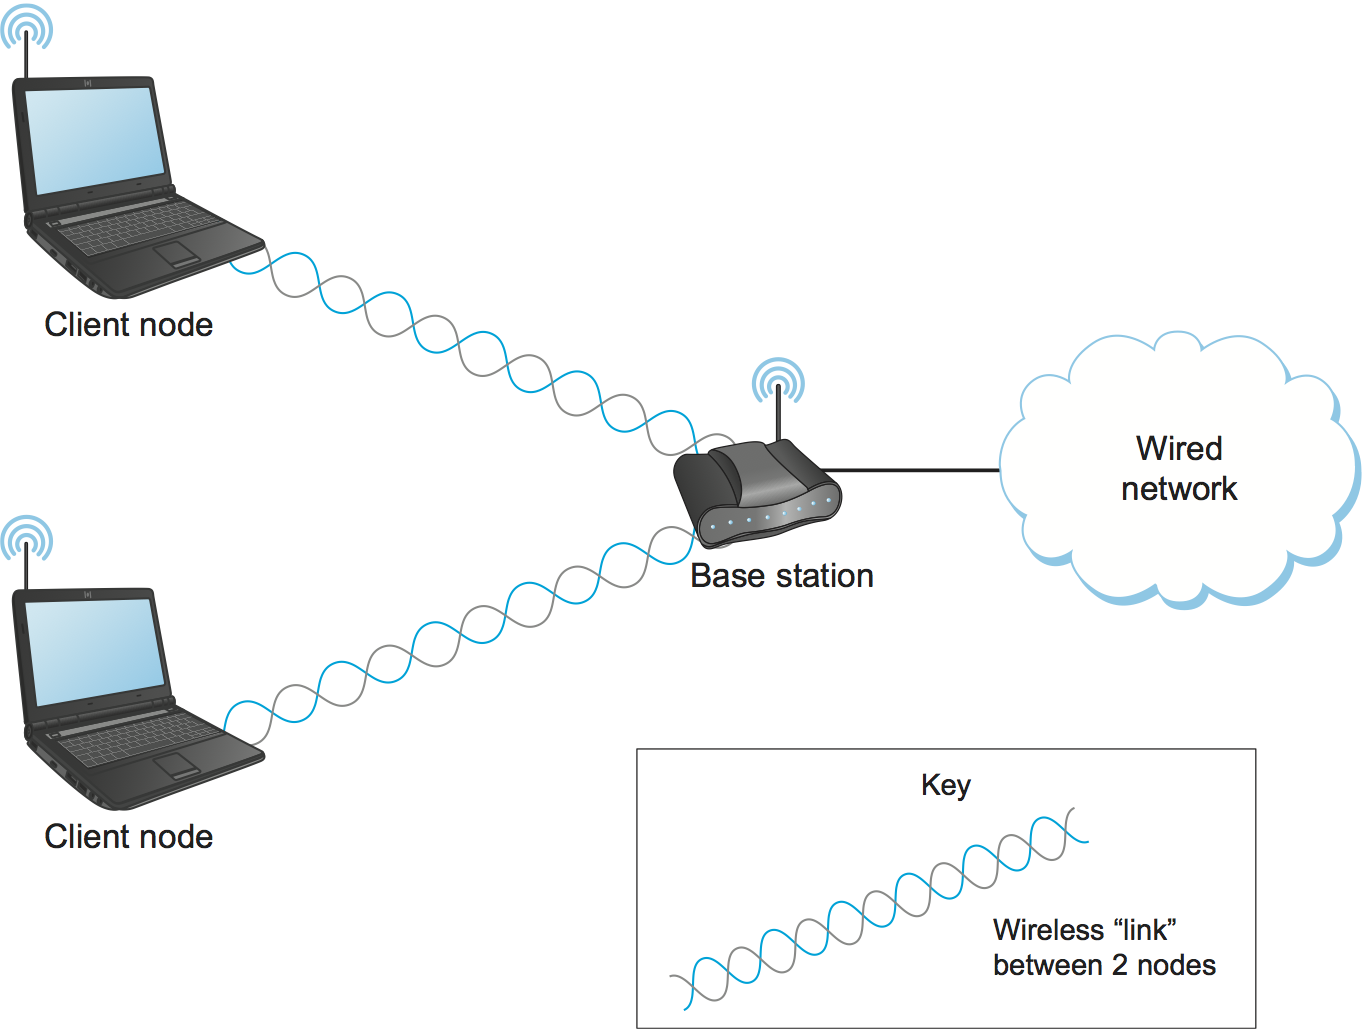
\includegraphics[width = 0.5\textwidth]{Pictures/Wireless base station.png}
        \caption{Caption}
        \label{fig:my_label}
    \end{figure}
    \item Access Point: Nodes form adhoc links between themselves, allowing direct communication.
    \begin{figure}[H]
        \centering
        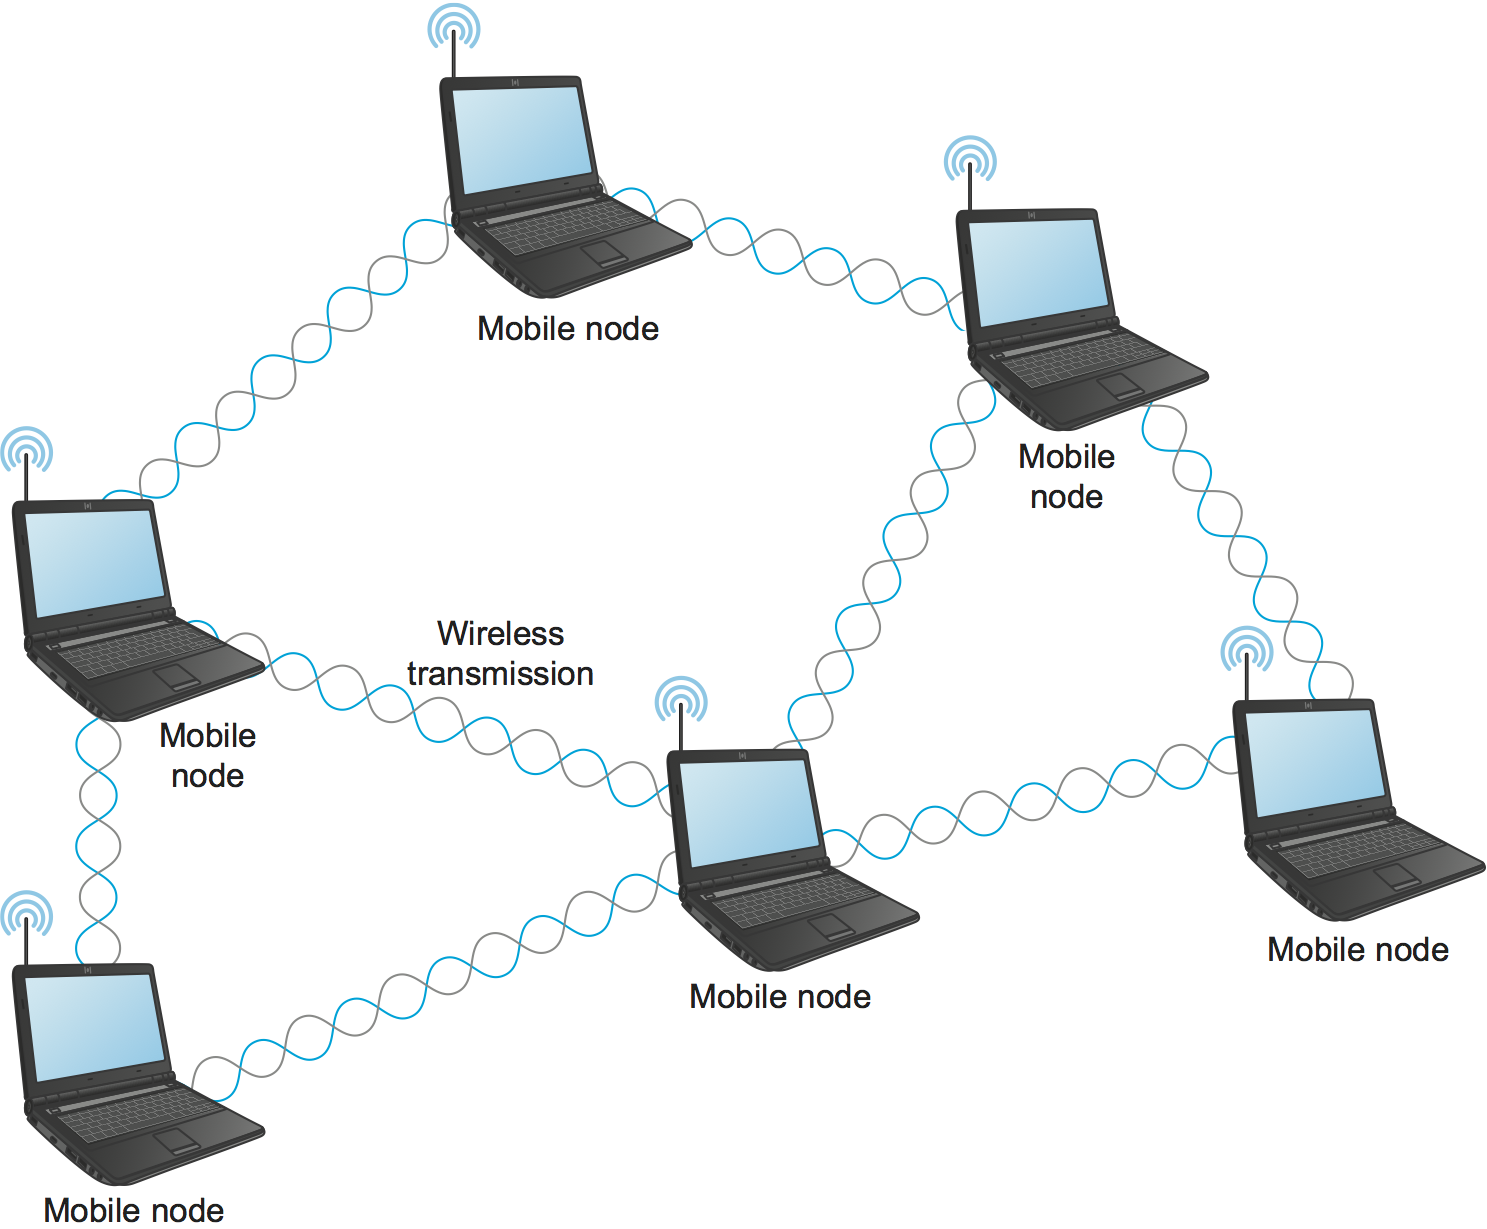
\includegraphics[width = 0.5\textwidth]{Pictures/Wireless mesh adhoc.png}
        \caption{Caption}
        \label{fig:my_label}
    \end{figure}
\end{enumerate}

\subsection{Current Wifi}
The technology today allows for greater speed and bandwidths. It is worth noting that while all the 802.11 standards define a maximum bit rate that can be supported, they mostly support lower bit rates as well (e.g., 802.11a allows for bit rates of 6, 9, 12, 18, 24, 36, 48, and 54 Mbps). At lower bit rates, it is easier to decode transmitted signals in the presence of noise. Different modulation schemes are used to achieve the various bit rates. In addition, the amount of redundant information in the form of error-correcting codes is varied. More redundant information means higher resilience to bit errors at the cost of lowering the effective data rate (since more of the transmitted bits are redundant). Since this is factual, read from the book.

\subsection{Collision Avoidance}
Two problems:
\begin{enumerate}
    \item Hidden Node Problem:
    \begin{figure}[H]
        \centering
        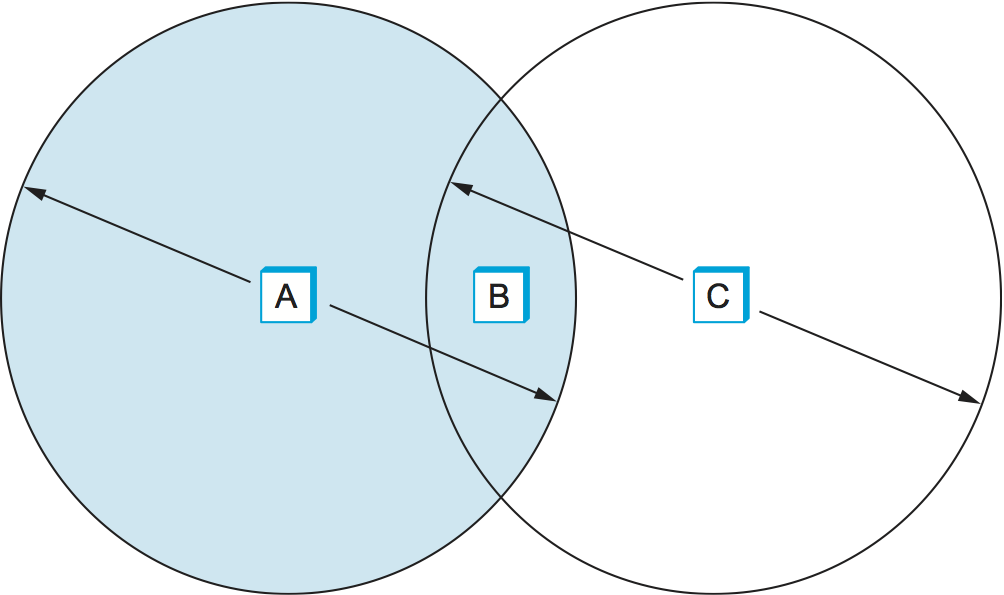
\includegraphics[width = 0.5\textwidth]{Pictures/hidden node.png}
        \label{fig:my_label}
    \end{figure}
    A hidden from C. A and C both want to communicate with B, the message collides, but unlike Ethernet where jamming sequence could be send, A and C are not within each other's range, so they cannot communicate each other's collision to each other.
    \item Exposed Node Problem:
    \begin{figure}[H]
        \centering
        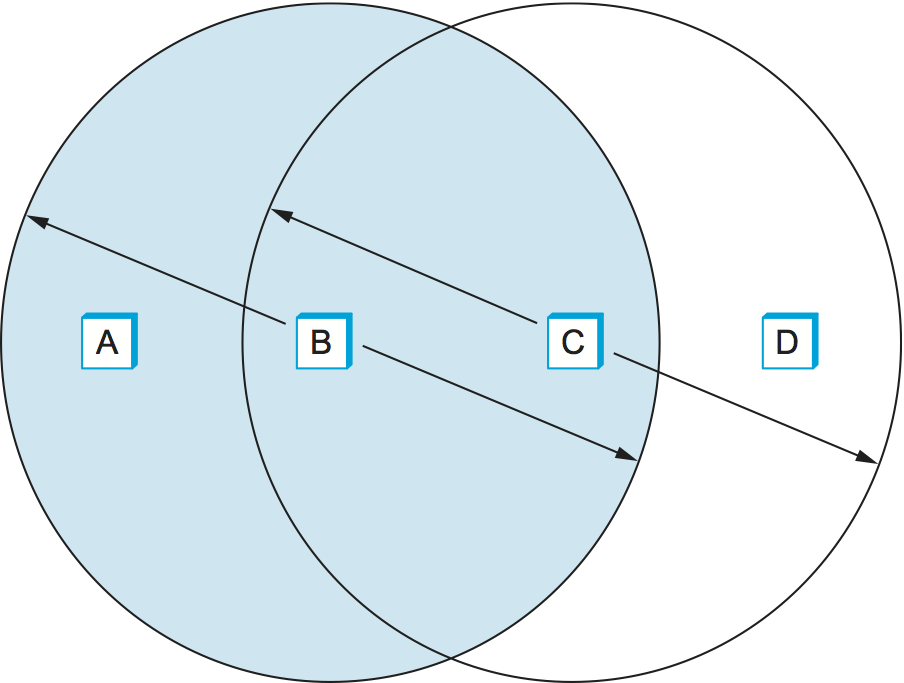
\includegraphics[width = 0.5\textwidth]{Pictures/exposed node.png}
        \label{fig:my_label}
    \end{figure}
    B wants to communicate with A and C wants to commuincate with D. They should be able to, but since B is in range of C or vice versa, if C is sending messsage to D, B thinks it can not send a message without interfering C,D is out of range of B, hence this is not an issue.
\end{enumerate}
\textbf{FIX}: 
\begin{enumerate}
    \item CSMA: The Carrier Sense part seems simple enough: Before sending a packet, the transmitter checks if it can hear any other transmissions; if not, it sends. However, because of the hidden node problem, just waiting for the absence of signals from other transmitters does not guarantee that a collision will not occur from the perspective of the receiver. For this reason, one part of CSMA/CA is an explicit ACK from the receiver to the sender. If the packet was successfully decoded and passed its CRC at the receiver, the receiver sends an ACK back to the sender.
    \item RTS-CTS. Ready to send, Clear to send. B sends message that it wants to send message to A, RTS. A receives it. A sends CTS to all in range. Those who are not A, then wait and don't send anything for the time allowed by the Wifi for one node to occupy the signal. If it does not receive CTS, but perhaps receives the RTS, then this node is free to talk to some other node, in problem of Exposed Node, D never receives a CTS from A, so it sends it's CTS to C, in response to C's RTS (which could have been sent before B started transmitting to A), and C sends message to D successfully.
    \item Obviously Collisions of RTS are possible, but if CTS is not received after a while, the nodes can always try again later on, using exponential backoff.
\end{enumerate}

\subsection{Distribution System}
These are used by AP's as mentioned above.
\begin{enumerate}
    \item Nodes can talk to nodes in range. What about outside? They talk to Distribution network, and node is sent to the node which far, but connected to the Wifi.
    \item \textbf{What if the node is moving?}
    \begin{enumerate}
        \item The node sends a Probe frame.
        \item All APs within reach reply with a Probe Response frame.
        \item The node selects one of the access points and sends that AP an Association Request frame.
        \item The AP replies with an Association Response frame.
    \end{enumerate}
    A node engages this protocol whenever it joins the network, as well as when it becomes unhappy with its current AP. This might happen, for example, because the signal from its current AP has weakened due to the node moving away from it. Whenever a node acquires a new AP, the new AP notifies the old AP of the change (this happens in step 4) via the distribution system.
\end{enumerate}

\subsection{Wifi Frame Format}
\begin{figure}[H]
    \centering
    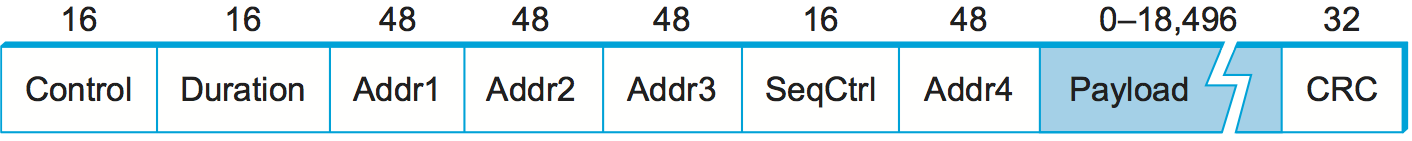
\includegraphics[width = \textwidth]{Pictures/Wifi Frame Format.png}
    \caption{Caption}
    \label{fig:my_label}
\end{figure}
The peculiar thing about the 802.11 frame format is that it contains four, rather than two, addresses. How these addresses are interpreted depends on the settings of the ToDS and FromDS bits in the frame’s Control field. This is to account for the possibility that the frame had to be forwarded across the distribution system, which would mean that the original sender is not necessarily the same as the most recent transmitting node. Similar reasoning applies to the destination address. In the simplest case, when one node is sending directly to another, both the DS bits are 0, Addr1 identifies the target node, and Addr2 identifies the source node. In the most complex case, both DS bits are set to 1, indicating that the message went from a wireless node onto the distribution system, and then from the distribution system to another wireless node. With both bits set, Addr1 identifies the ultimate destination, Addr2 identifies the immediate sender (the one that forwarded the frame from the distribution system to the ultimate destination), Addr3 identifies the intermediate destination (the one that accepted the frame from a wireless node and forwarded it across the distribution system), and Addr4 identifies the original source. Like a traceback.

\subsection{Bluetooth}
Slave Devices, Master Devices. Slave Devices can not talk to each other. Bluetooth operates in the license-exempt band at 2.45 GHz. Bluetooth links have typical bandwidths around 1 to 3 Mbps and a range of about 10 m. For this reason, and because the communicating devices typically belong to one individual or group, Bluetooth is sometimes categorized as a Personal Area Network (PAN). Parked devices, and active devices. Once parked can only reactivated by the master device.

\chapter{Chapter 3: Internetworking}

\section{Switching Basics}
How to interconnect nodes on different networks?
\begin{enumerate}
    \item Connect the switch of the two networks. This is the most usual practice.
\end{enumerate}
What do we need for networks to communicate?
\begin{enumerate}
    \item Every node needs an address that can at the very least be uniquely identified on the network itself.
    \item In reality, the Ethernet addresses are distributed to companies, so the Ethernet address are globally unique. So, the hardware is uniquely identifiable.
    \item We need to be able to identify who is connected where, and when we send data, through which it is the best idea to send it through. This is the concept of forwarding table.
\end{enumerate}

\subsection{Datagrams}
\begin{enumerate}
    \item Called connection-less way of making networks. 
    \item Each router has a forwarding table (also called routing table), and when a packet comes to it, it just checks where it needs to go, and sends it there. 
    \item This requires the data-gram to have the entire address details to be in the packet, otherwise some node may send it to the wrong place. 
    \item This is good when topology is shifting too much and pre planning route is very hard. The responsibility is shifted to the router(switch) to find the path. 
    \item Since there is no pre-planning, no way to know if packet can be delivered. This is similar to how packet switching works.
\end{enumerate}


\subsection{Virtual Circuit Switching}
\begin{enumerate}
    \item This is called a connection oriented connection.
    \item  The network administrator, or the nodes themselves communicate to fix connection routes.
    \item One RTT is spent making sure connection is possible.
    \item Each switch has a table for every connection it has seen or is pre loaded. The table looks like this:
    \begin{table}[H]
        \centering
        \begin{tabular}{ | c | c | c | c |}
        \hline
        Incoming Interface & Incoming VCI & Outgoing Interface & Outgoing VCI \\
        \hline
        2 & 5 & 1 & 11 \\
        \hline
        \end{tabular}
        \caption{VCI}
        \label{tab:VCI Table}
    \end{table}
    \item Every connection is identified using the VCI. So every switch maps the receiving VCI from an interface to an outgoing one and then sends it to the corresponding port. This is repeated until the last node. Usually numbering starts from 0 at each switch, if 0 is taken then we increment and define a map using the received VCI and port (interface) to the new incremented VCI and interface pair.
    \item This is good when topology does not change a lot, path stay there. Little overhead, as complete address not needed.
    \item ATM (Asynchrous Transfer Mode) is a nice example.
\end{enumerate}

\subsection{Source Routing}
\begin{enumerate}
    \item One last way that networks can communicate is that the source node tells where the packet needs to go, dictating each hop from the source itself at each switch.
    \item It is obvious the problems we can see. Topology shifts, the node needs to have the entire knowledge if the network, that is possible only if everyone is talking to each other ALL the time. Inefficient.
    \item This can be implemented by reshuffling, stripping and pointers.
    \item Source routes are sometimes categorized as strict or loose. 
    \begin{enumerate}
        \item In a strict source route, every node along the path must be specified as mentioned above, whereas 
        \item a loose source route only specifies a set of nodes to be traversed, without saying exactly how to get from one node to the next. A loose source route can be thought of as a set of waypoints rather than a completely specified route. The loose option can be helpful to limit the amount of information that a source must obtain to create a source route.
    \end{enumerate}
\end{enumerate}

\section{Switched Ethernet}
\subsection{Learning Bridge}
As someone sends to me, I learn where the guy is connected. No need to flood.

\subsection{Spanning Tree}
The network can be seen as a planar graph, from which a spanning tree can be determined. The algorithm can be summarised as:
\begin{enumerate}
    \item Functional switch with lowest ID is the root.
    \item Every node which sees all offers form other nodes, chooses the strictly smallest one.
    \item Every node which sees two switches offering same distance from the root, it chooses the switch with lower ID.
    \item If two switches see they have same distance from the root, the close connection between themselves.
    \item If creation of path creates a cycle, don't create connection.
    \item If all nodes covered, stop.
\end{enumerate}
\subsection{VLAN}
These things are not exactly scalable. Imagine flooding a really big network. The solution to do this is augment the network into smaller virtual networks, Instead of the entire network knowing everything about the entire network, it knows more about the small partitions. Then whenever the packet wants to talk to other nodes, in these other virtual networks, the packet is passed and then the that network takes care of it. Obviously more information is added into the header. Uses learning bridges. Packet forwarding does not alter IP or MAC, nothing.

\section{Internet IP}
\subsection{Service Model}
Internet protocol is connection less service. This is called best-effort as well. Since connection less, we have datagrams.

\subsection{IPv4 Packet Format}
\begin{figure}[H]
    \centering
    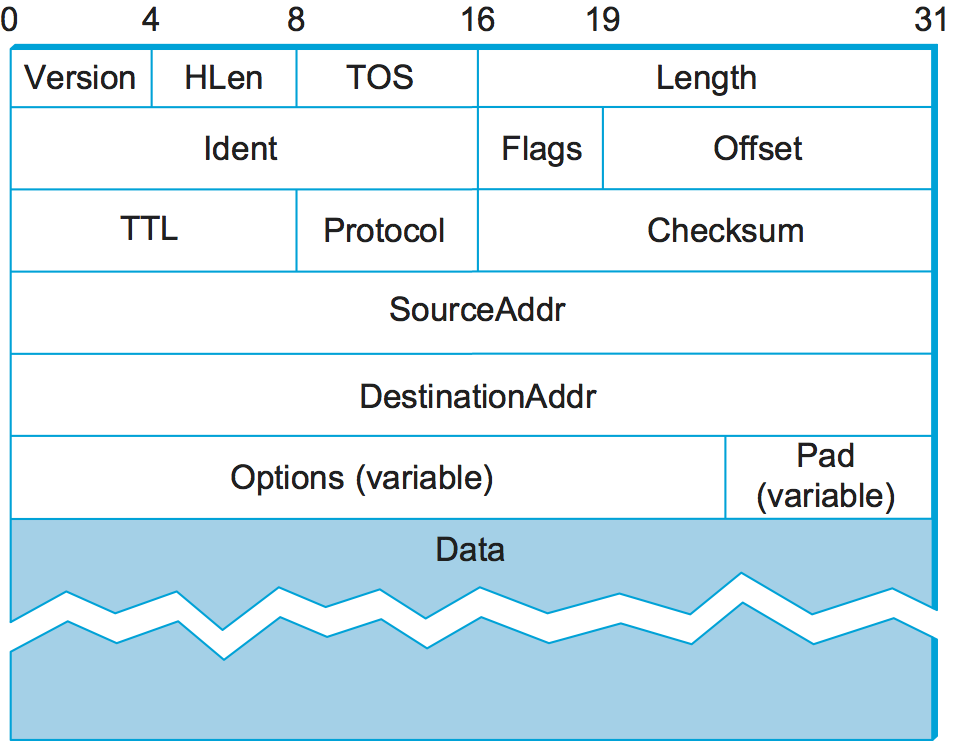
\includegraphics[width = \textwidth]{Pictures/ipv4.png}
    \caption{Packet Format}
    \label{fig:my_label}
\end{figure}

\subsection{Fragmentation and Reassembly}
Never reassemble at the intermediate switch.
\begin{figure}[H]
    \centering
    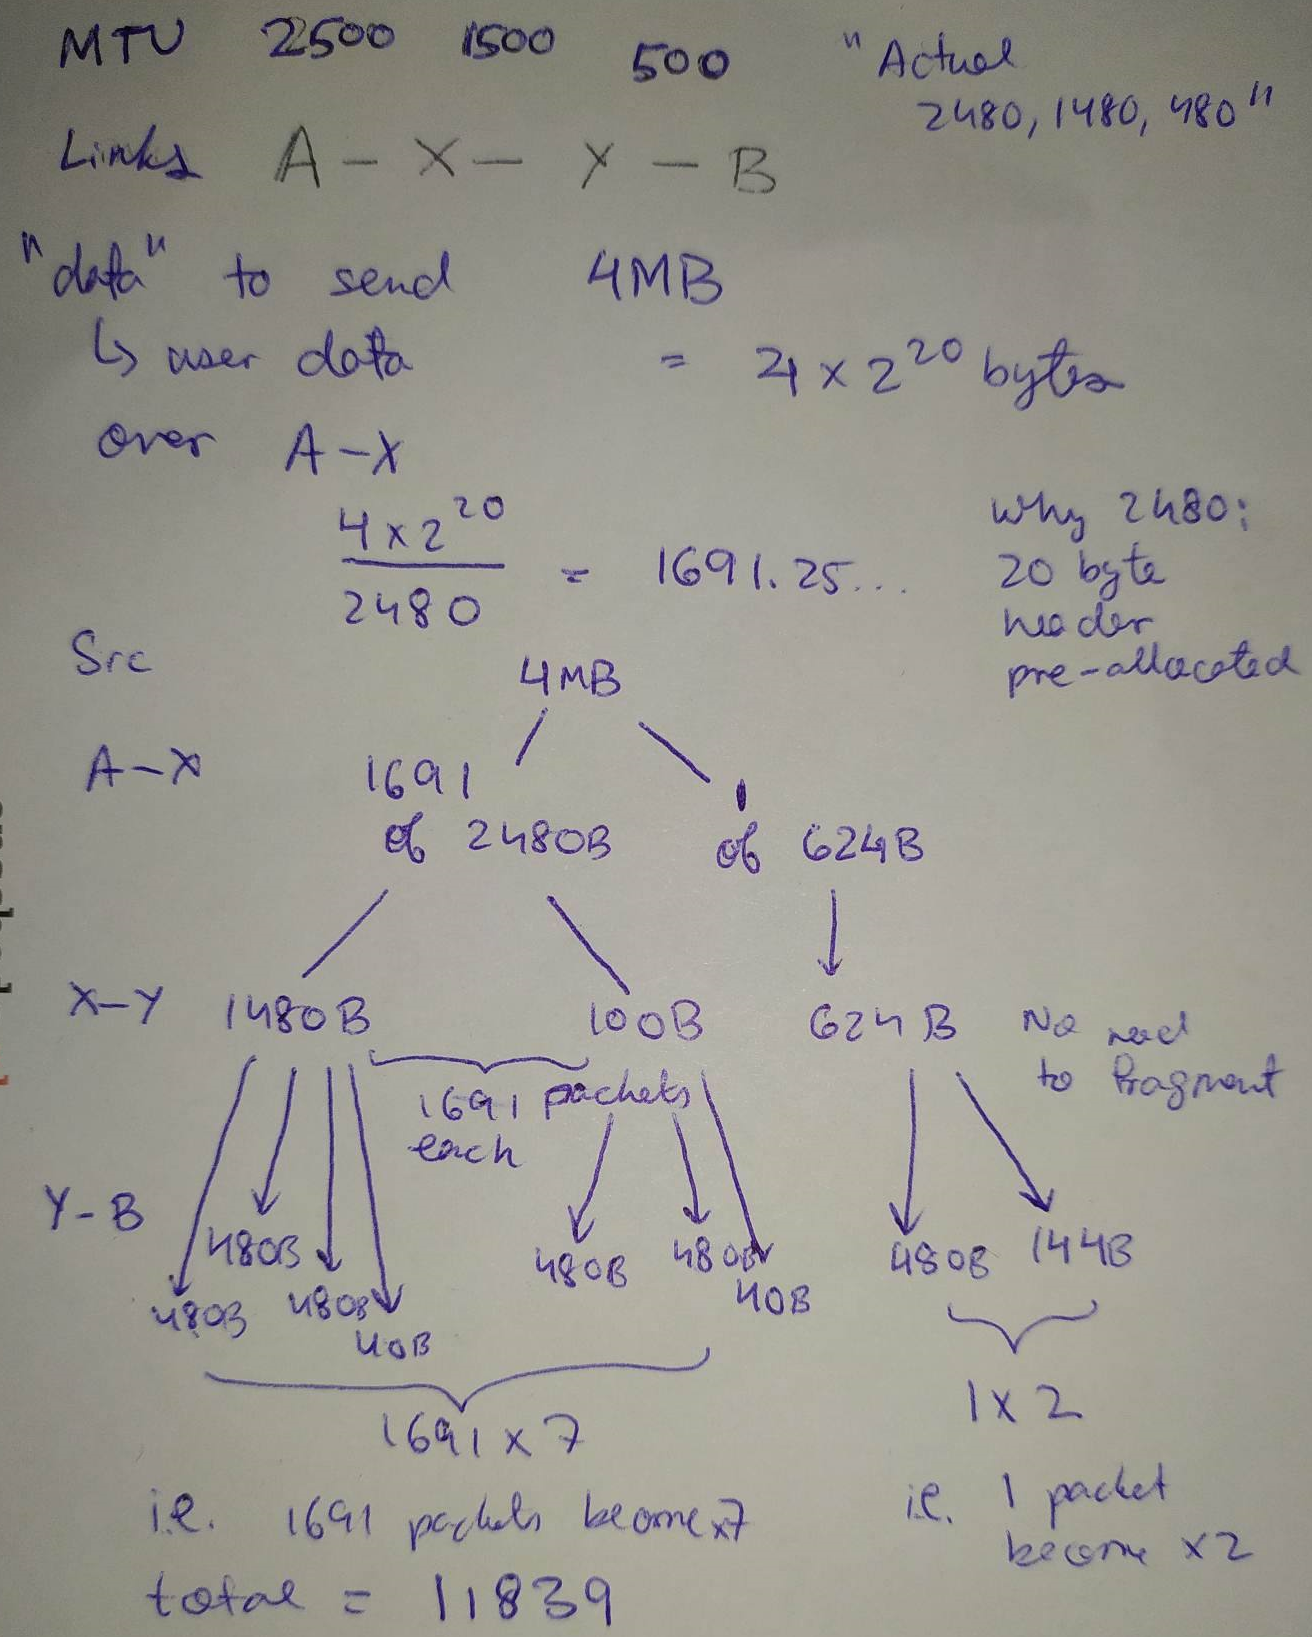
\includegraphics[width = \textwidth]{Pictures/MTU fragmentation.png}
    \caption{Example - all you need}
    \label{fig:example}
\end{figure}

\subsection{Global Addressing}
\begin{figure}[H]
    \centering
    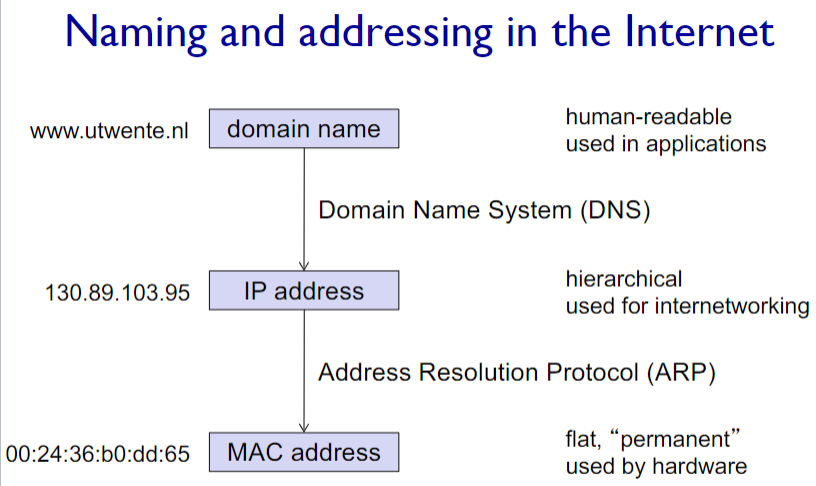
\includegraphics[width = \textwidth]{Pictures/Addressing.png}
    \caption{Addressing}
    \label{fig:my_label}
\end{figure}
\subsection{Datagram forwarding in IP}
\begin{enumerate}
    \item You have the datagram.
    \item it has an address.
    \item compare in the routing table, do I know how to get there?
    \begin{enumerate}
        \item Yes it on my network: Send to that node
        \item No: Send to best router, the next hop.
        \begin{enumerate}
            \item in case many routers, choose best one.
        \end{enumerate}
        \item in case no best router, absolutely no idea, give to default router.
    \end{enumerate}
\end{enumerate}

\subsection{Classful Addressing, Classless Addressing, Subnetting}
\begin{enumerate}
    \item Subnetting: \\
    ex: 216.3.128.128 (/25)-- this means the 25 MSB are network address. The rest is host address.//
    The mask is: 255.255.255.240 come from binary (11111111111111111111111110000000)
    \begin{enumerate}
        \item ex. 216 .   3 . 128 . (1000 0010)
        \item To get network address: received address (AND) subnet mask
        \item compare with the first 25 bits. If they same, then on this network, so extract host address (XOR) do whatevs. this case it is 2.
        \item if not, then we are in the wrong place send it away.
    \end{enumerate}
    \item Classful:
    \begin{enumerate}
        \item Class A, B, C: basically subnets with /8, /16, /24.
    \end{enumerate}
    \item CIDR: Classless Interdomain Routing.\\
    Think of Classful Addressing as a special case CIDR.
    The example of sub netting explains what happens.
    \item Last topic, Network Migration.
    Using a mask, we can add another 1, i.e. /25 to /26. Using this we can define sub networks, like a tree hierarchy. But if one of them wants to leave, they take their address, and then the switch broadcasts that specific chunk of address. When packets are being sent, the longest prefix matching is used first, since it more specific.
    \begin{figure}[H]
        \centering
        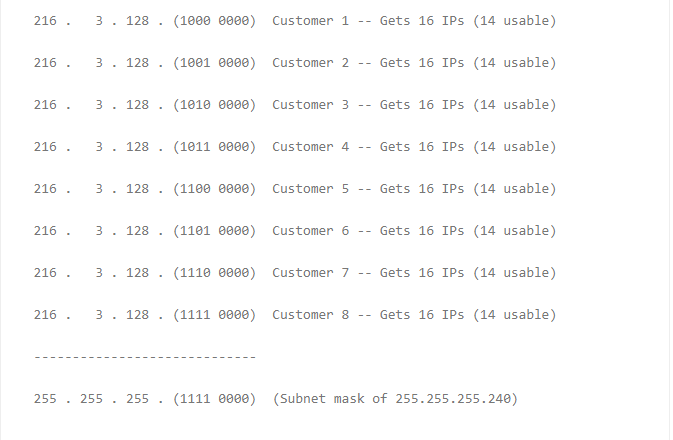
\includegraphics[width = \textwidth]{Pictures/Subnet.png}
        \caption{Subnet: The first address would then have a mask of /28 since the first 4 0's are fixed. If that network migrates this address is removed, but the switch still broadcasts the previous address. No change there. If someone wants to send a packet, they send to the one with the highest prefix /28, hence that's where the packet is sent first.}
        \label{fig:my_label}
    \end{figure}
\end{enumerate}
\subsection{DHCP}
Give the host, an address. Dynamic Host Resolution Protocol.

\subsection{ARP}
Address Resolution Protocol. Get the MAC to know where to send the data, so the actual party can identify on the Data link layer it needs to compare the MAC. In this we look at the IP address and check to which router or the node itself I need to send the packet to. So when packets travel over many routers, of different LANs, the MAC addresses change since they are travelling between routers and then finally the node. In case bridges are used, nothing changes, as the the same network is simply broken into many parts and not entirely different networks exist. In the same network the bridges know where to send each MAC.

\subsection{Routing}
\begin{enumerate}
    \item RIP: Routing Information Vector. IE Distance vector- Bellman Ford algorithm.
    \item OSPF: Open Shortest Path First. Link State Routing. IE Dijkstra algorithm.
    \item AH OD VR: Ad hoc on demand vector routing. Mobile phones. Dynamic networks- too many changes, too much movement. The routes are made, fixed only when needed as the name suggests, so the orutes are not presistent for too long, which is good for the shifting topology.
\end{enumerate}

\chapter{Chapter 4: Advanced Internetworking}
\section{Interdomain routing}
\subsection{Border Gateway Protocol (BGP)}
\begin{enumerate}
    \item Problem: I do not want to provide a route through me, if I am paying. I want to be able to choose a route which is cheaper, maybe faster, maybe more secure. How can this be done?
    \item How it is done:
    \textbf{Autonomous Systems}: These are "systems" which represent a network or access to a network. Every ISP can have many (AS) and every AS can have many access points. AS can even connect to one another.
    \begin{enumerate}
        \item Stub AS: Only one access point AS
        \item Multihomed-AS: Multiple AP's. Helps to have redundancy, have connections in many geographic areas, need to connect them.
        \item Transit AS: their main purpose is ti send data across two or more AS, or happen to provide this service along with other services.
    \end{enumerate}
    \item \textbf{The purpose of BGP}: First, it is necessary to find some path to the intended destination that is loop free. Second, paths must be compliant with the policies of the various autonomous systems along the path—and, as we have already seen, those policies might be almost arbitrarily complex. Thus, while intradomain focuses on a well-defined problem of optimizing the scalar cost of the path, interdomain focuses on finding a non-looping, policy-compliant path—a much more complex optimization problem.
    \item \textbf{How does all this help us to build scalable networks?}
    \begin{enumerate}
        \item First, the number of nodes participating in BGP is on the order of the number of autonomous systems, which is much smaller than the number of networks.
        \item Second, finding a good interdomain route is only a matter of finding a path to the right border router, of which there are only a few per AS. Thus, we have neatly subdivided the routing problem into manageable parts, once again using a new level of hierarchy to increase scalability.
    \end{enumerate}
    \item The complexity of interdomain routing is now on the order of the number of autonomous systems, and the complexity of intradomain routing is on the order of the number of networks in a single AS.
    \item \textbf{How can the nodes inside a AS use the links?}
    \begin{enumerate}
        \begin{figure}[H]
            \centering
            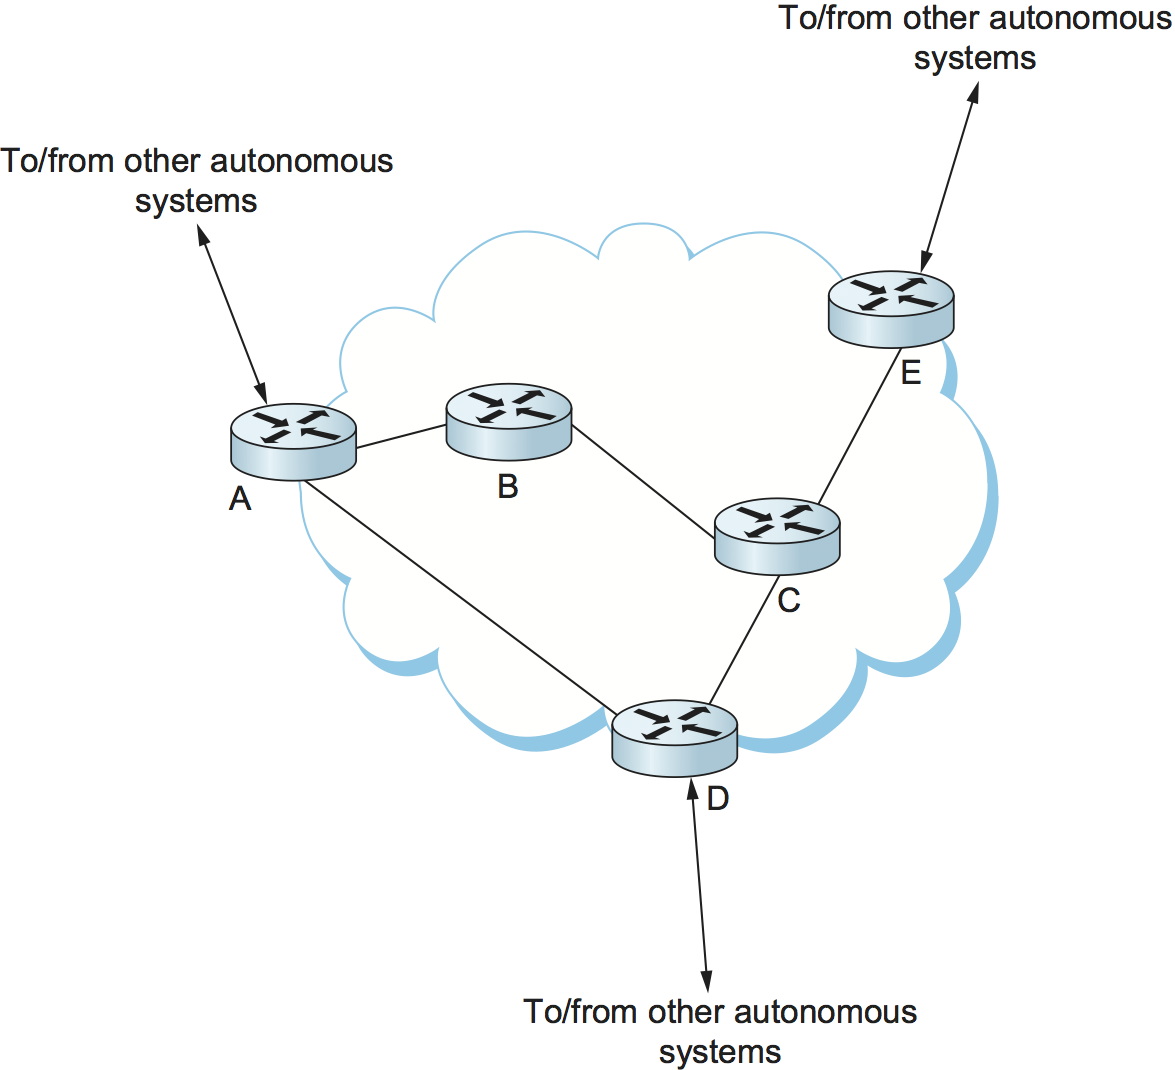
\includegraphics[width = 0.5\textwidth]{Pictures/bgp.png}
            \caption{Example of interdomain and intradomain routing. All routers run \textbf{i}BGP (OSPF or DV) and an intradomain routing protocol \textbf{e}BGP. Border routers A, D, and E also run \textbf{e}BGP to other autonomous systems.}
        \end{figure} 
        \item \textbf{interior} BGP: OSPF or DV
        
        \item \textbf{exterior} BGP: the actual BGP
    \end{enumerate}
\end{enumerate}

\section{IPv6}

IPv6 provides a 128-bit address space, as opposed to the 32 bits of version 4. Thus, while version 4 can potentially address 4 billion nodes if address assignment efficiency reaches 100\%, IPv6 can address 3.4 × 1038 nodes, again assuming 100\% efficiency.

\subsection{Host Density}
Max threshold for host density is 87.5\%. This is where it starts getting problematic.
\begin{figure}[H]
    \centering
    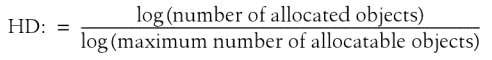
\includegraphics[width = \textwidth]{Pictures/Host Density.png}
    \caption{Host Density Formula}
    \label{fig:my_label}
\end{figure}

\subsection{Desirable Features of IPv6}
\begin{enumerate}
    \item Support for real-time services
    \item Security support
    \item Autoconfiguration (i.e., the ability of hosts to automatically configure themselves with such information as their own IP address and domain name)
    \item Enhanced routing functionality, including support for mobile hosts
\end{enumerate}

\subsection{Address Notation}
\begin{enumerate}
    \item 8 pieces of 16 bits represented by 4 Hexadecimals.
    \item Just as with IPv4, there is some special notation for writing down IPv6 addresses. The standard representation is x:x:x:x:x:x:x:x, where each x is a \textbf{hexadecimal} representation of a \textbf{16-bit} piece of the address. An example would be: \\47CD:1234:4422:ACO2:0022:1234:A456:0124.
    \item Any IPv6 address can be written using this notation. Since there are a few special types of IPv6 addresses, there are some special notations that may be helpful in certain circumstances. For example, an address with a large number of contiguous 0s can be written more compactly by omitting all the 0 fields. Thus, 47CD:\textbf{0000:0000:0000:0000:0000}:A456:0124 could be written 47CD\textbf{::}A456:0124
    \item Clearly, this form of shorthand can only be used for \textbf{one} set of contiguous 0s in an address to avoid ambiguity.
\end{enumerate}

\subsection{Route Aggregation}
IPv6 is classless, so implements CIDR as well. But, since there are so many addresses we have more hierarchy in the way the addresses are assigned. At the moment 001 prefix address are only assigned, whch means we still have 87.5\% addresses left that have not yet even been touched.

\begin{figure}[H]
    \centering
    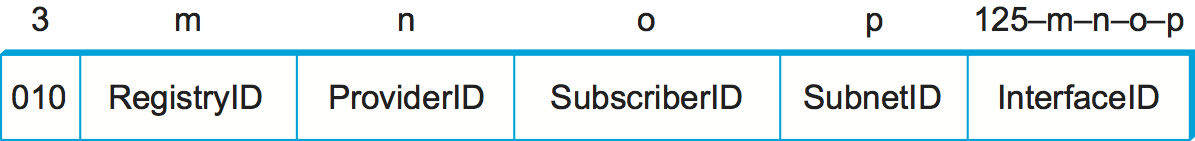
\includegraphics[width = \textwidth]{Pictures/ipv6 format when assigned.png}
    \caption{An IPv6 provider-based unicast address.}
    \label{fig:my_label}
\end{figure}
Problem may occur when two people connected tot he same router, but a go around is to broadcast both addresses to this and that part of the world, to create redundancy, and reduce load even.

\subsection{Packet Format}
Even though ipv6 is more complex the header is simpler. It has a header length of 40bytes, despite the fact the addresses are 4 times as long. This is pretty nice, and is possible since people took notice of what protocol were quite redundant and not needed in ipv6.

\begin{figure}[H]
    \centering
    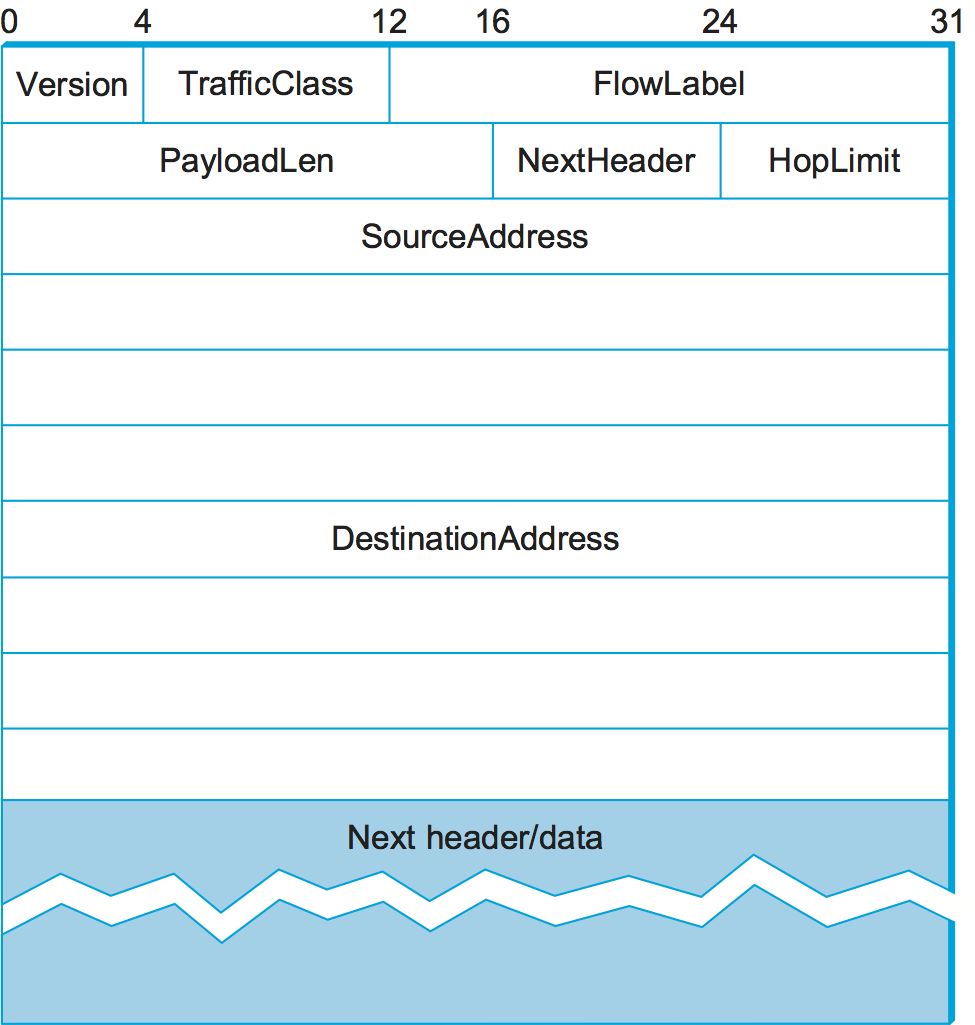
\includegraphics[width = \textwidth]{Pictures/ipv6 packet fomrat.png}
    \caption{ipv6 packet format}
    \label{fig:my_label}
\end{figure}


\subsection{Advanced Capabilities}
\begin{enumerate}
    \item Autoconfiguration: for IPv4 we always needed a DHCP. for IPv6 since the address sapce is so big we can any of these two:
    \begin{enumerate}
        \item Put your unique ethernet 48 bits into the interfaceID.
        \item choose one at random, with a space so big, it is likely unused.
    \end{enumerate}
    \item Source-Directed Routing: Another of IPv6’s extension headers is the routing header. In the absence of this header, routing for IPv6 differs very little from that of IPv4 under CIDR. The routing header contains a list of IPv6 addresses that represent nodes or topological areas that the packet should visit en route to its destination. The reason are same as discussed in BGP.
\end{enumerate}

\section{Multicast}
Normal IP communication, in which each packet must be addressed and sent to a single host, is not well suited to such applications. If an application has data to send to a group, it would have to send a separate packet with the identical data to each member of the group. This redundancy consumes more bandwidth than necessary. IP multicast is more scalable because it eliminates the redundant traffic (packets) that would have been sent many times over the same links, especially those near to the sending host.

\textbf{Types of Multicast}
\begin{enumerate}
    \item \textbf{Source Specific Multicast (SSM):} a receiving host specifies both a multicast group and a specific sending host. The receiving host would then receive multicasts addressed to the specified group, but only if they are from the specified sender.
    \item \textbf{Any Source Multicast (ASM):} many IP to many IP, so part of group but any sender.
\end{enumerate}

\textbf{How to join a group?}
\begin{enumerate}
    \item IPv4, that protocol is the Internet Group Management Protocol (IGMP)
    \item IPv6, it is Multicast Listener Discovery (MLD).
\end{enumerate}
For both they need to communicate with the router to become a part of the group. The router then does polling periodically to check is the node is still interested in the group, or has crashed, left correctly, etc.

As said before in IPv6 we have multicast addresses so deos IPv4.

\section{Multicast Routing}
As all thing uni and packets, Multicast needs routing too.
\begin{enumerate}
    \item \textbf{Distance Vector Multicast Routing Protocol (DVMRP):} If I get packet from Source S, and I get it from the best path, I send to all. This floods the network and this is bad. If the packet then comes from not the bes tnode, sine flooding is happening, I do not forward that.
    Another problem people who are not part of the group G, need to send I don't part of this. For this we have the next one, \textbf{Sparse Mode}.
    \item \textbf{Protocol Independent Multicast - Sparse Mode (PIM-SM):}  Basically, I ask to join using a Randevouz Point, then a specific tree is created for this group for the router.
    \begin{figure}[H]
        \centering
        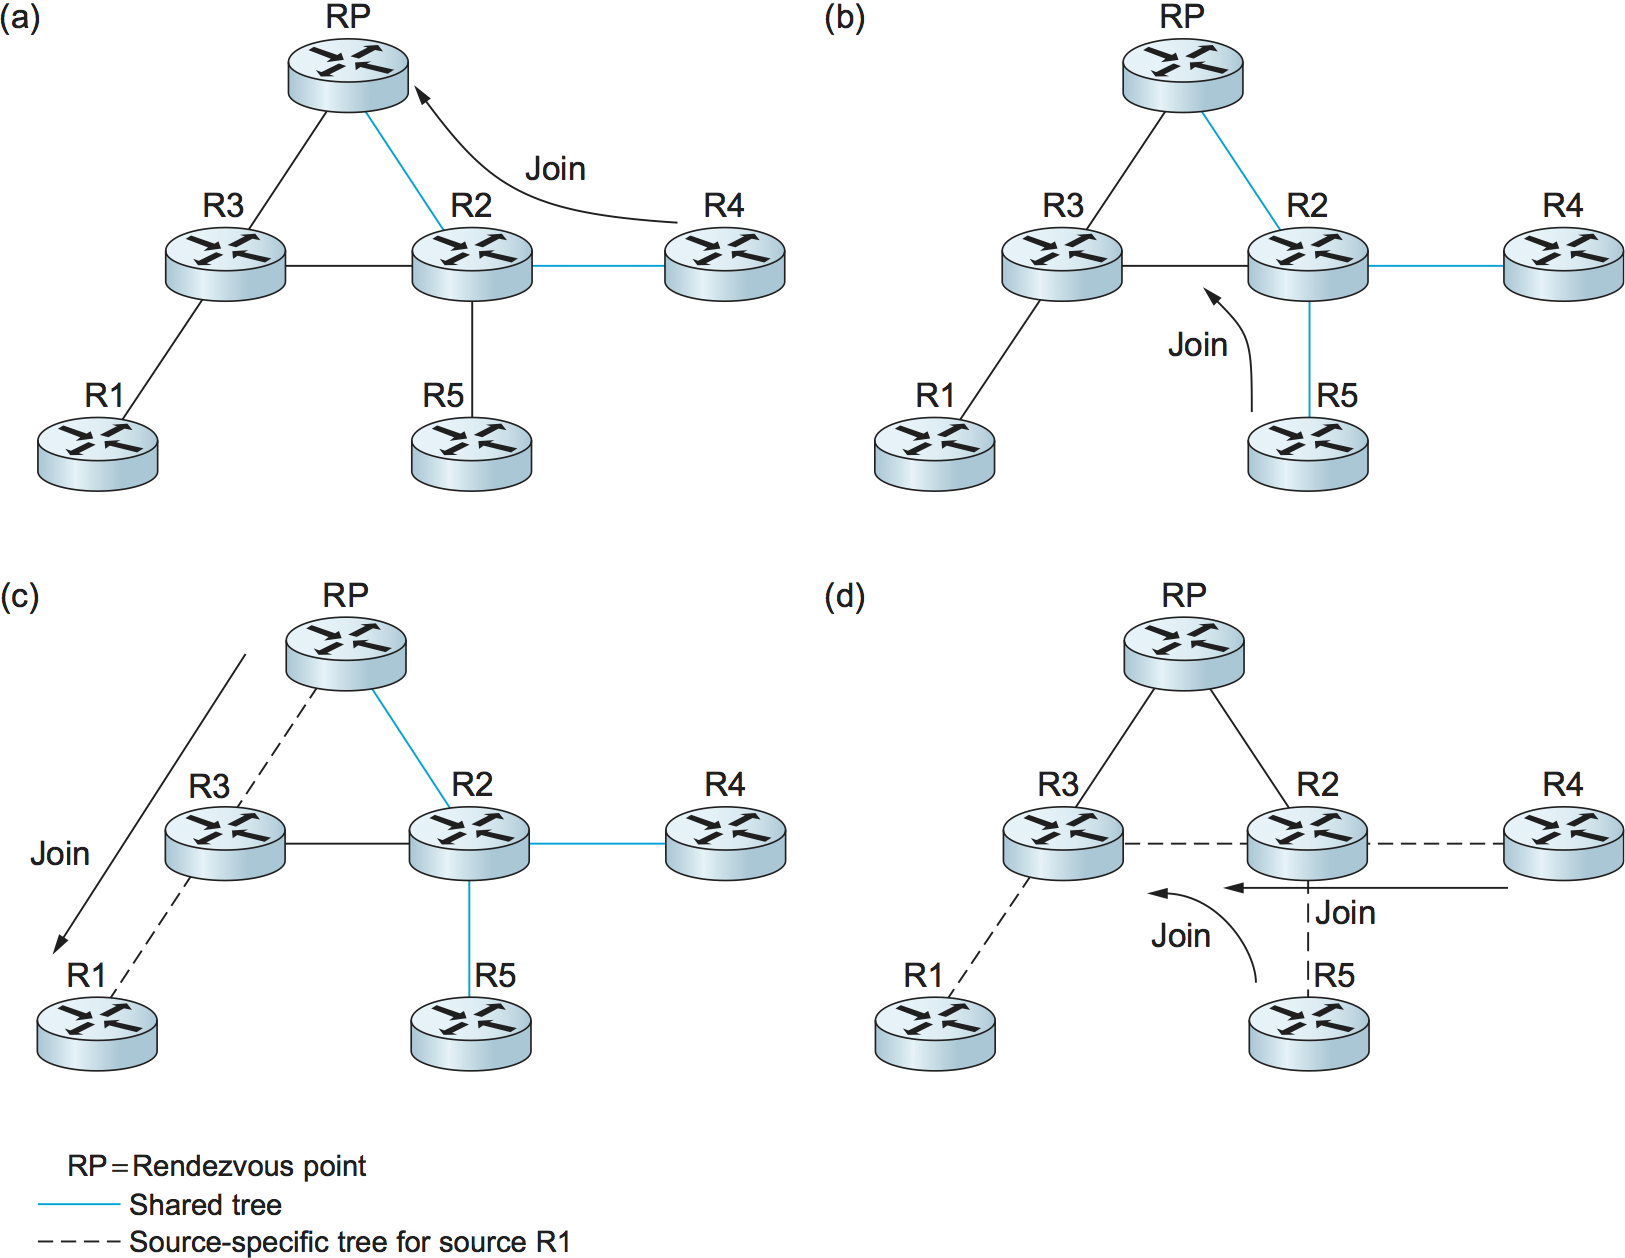
\includegraphics[width = \textwidth]{Pictures/PIM-SM.png}
        \caption{PIM operation: (a) R4 sends a Join message to RP and joins shared tree; (b) R5 joins shared tree; (c) RP builds source-specific tree to R1 by sending a Join message to R1; (d) R4 and R5 build source-specific tree to R1 by sending Join messages to R1.}
        If node wants to send to RP, the connecting router may choose to tunnel if it does not want others to know. Creating source specific tree when all nodes have joined and all.//
        \textbf{What if someone wants to send packet that is not even in the same network? Go to Interdomain Multicast}
    \end{figure}
    \item \textbf{Interdomain Multicast (MSDP):} To extend multicast across domains using PIM-SM, the Multicast Source Discovery Protocol (MSDP) was devised. Each RP has one or more MSDP peer RPs in other domains. Each pair of MSDP peers is connected by a TCP connection over which the MSDP protocol runs.
    Send message to RP to register as source. Handle intra domain requests using reverse path broadcasts. If on another netowrk, send message to RP on that network, which should have registered before, and then that node sends join. Accept and all of that thing. Meanwhile, the source keeps sending Source Active messages to tell others who would like to join. One all joined up create tree and send data.
    \item \textbf{Source-Specific Multicast (PIM-SSM):} 
    The introduction of PIM-SSM has provided some significant benefits, particularly since there is relatively high demand for one-to-many multicasting:
    \begin{enumerate}
    \item Multicasts travel more directly to receivers.
    \item The address of a channel is effectively a multicast group address plus a source address. Therefore, given that a certain range of multicast group addresses will be used for SSM exclusively, multiple domains can use the same multicast group address independently and without conflict, as long as they use it only with sources in their own domains.
    \item Because only the specified source can send to an SSM group, there is less risk of attacks based on malicious hosts overwhelming the routers or receivers with bogus multicast traffic.
    \item PIM-SSM can be used across domains exactly as it is used within a domain, without reliance on anything like MSDP.
    \item SSM, therefore, is quite a useful addition to the multicast service model.
    \end{enumerate}
    \item \textbf{Bidirectional Trees (BIDIR-PIM): } I only they are the same thing as the question that question which was weird and going both directions, i.e. bidirectional trees.
    
\end{enumerate}

\section{MobileIP}
\subsection{Definition}
\begin{enumerate}
    \item \textbf{Home network} The home network of a mobile device is the network within which the device receives its identifying IP address (home address).
    \item \textbf{Home address} The home address of a mobile device is the IP address assigned to the device within its home network.
    \item \textbf{Foreign Network} A foreign network is the network in which a mobile node is operating when away from its home network.
    \item \textbf{Care-of-Address} The care-of address of a mobile device is the network-native IP address of the device when operating in a foreign network.
    \item \textbf{Home Agent} A home agent is a router on a mobile node’s home network which tunnels datagrams for delivery to the mobile node when it is away from home. It maintains current location (IP address) information for the mobile node. It is used with one or more foreign agents.
    \item \textbf{Foreign Agent} A foreign agent is a router that stores information about mobile nodes visiting its network. Foreign agents also advertise care-of-addresses which are used by Mobile IP.
    \item \textbf{Binding} A binding is the association of the home address with a care-of address.
\end{enumerate}

\subsection{How work?}
So if I am sending a packet and I am not home, I send it to my agent, and he sends it to the node I wanted to send to, often using tunneling, i.e. it encapsulates my packet and sends it. If someone tries to send a packet to me, they send it to my home, then the home agent there tunnels the packet to my foreign agent who sends it to me, when I am away. This obviously requires a lot of registration.
\begin{figure}[H]
    \centering
    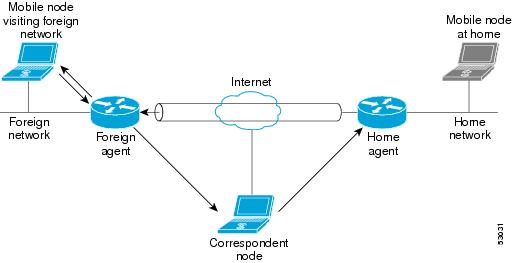
\includegraphics[width = \textwidth]{Pictures/MobileIPSending.jpg}
\end{figure}
When a packet finally arrives at the foreign agent, it strips the extra IP header and finds inside an IP packet destined for the home address of the mobile node.
\par
What about traffic in the other direction (i.e., from mobile node to fixed node)? This turns out to be much easier. The mobile node just puts the IP address of the fixed node in the destination field of its IP packets while putting its permanent address in the source field, and the packets are forwarded to the fixed node using normal means. Of course, if both nodes in a conversation are mobile, then the procedures described above are used in each direction.

\chapter{Chapter 5: End-to-End protocols}

\section{UDP}
Simple Demultiplexor - user Datagram Protocol. There are likely to be many processes running on any given host, so the protocol needs to add a level of demultiplexing, thereby allowing multiple application processes on each host to share the network.

\textbf{How to know demultiplex?}
\begin{enumerate}
    \item \textbf{OS assigned process Id (pid):} Typically not used since it is practical if a centralised system was in charge of all requests.
    \item \textbf{Port numbers: } More typically used.
    \begin{enumerate}
        \item There is a demultiplexing function contains an identifier port for both sender and receiver. Ususally 16 bits long each. This allows for $2^{16}$ port numbers, enough for a single node. Hence the \textbf{port}, \textbf{host} pair is used to identify this connection.
        \item \textbf{How to know to which port to send to?}
        \begin{enumerate}
            \item Agree before hand. Called the well-known port. For HTML requests port 80 is generally used, for DNS requests port 53, and so on. If busy, retry later or send to some secondary agreed port. They can different from OS to OS. They can be changed during the conversation, for example- initiate using a well known one, and then switch to someother to allow others to talk on the well known one.
            \item Use a port mapper. Think of hash tables, for asking to which port should I send a message. The advantage is that we don;t have to rely on port 80 to be the fixed one forever, can change anytime without changing the protocol.
        \end{enumerate}
    \end{enumerate}
        \item \textbf{How demultiplexed?: }  
    No flow control, if there is no space in the queue, just throw away the packet.
    \begin{figure}[H]
        \centering
        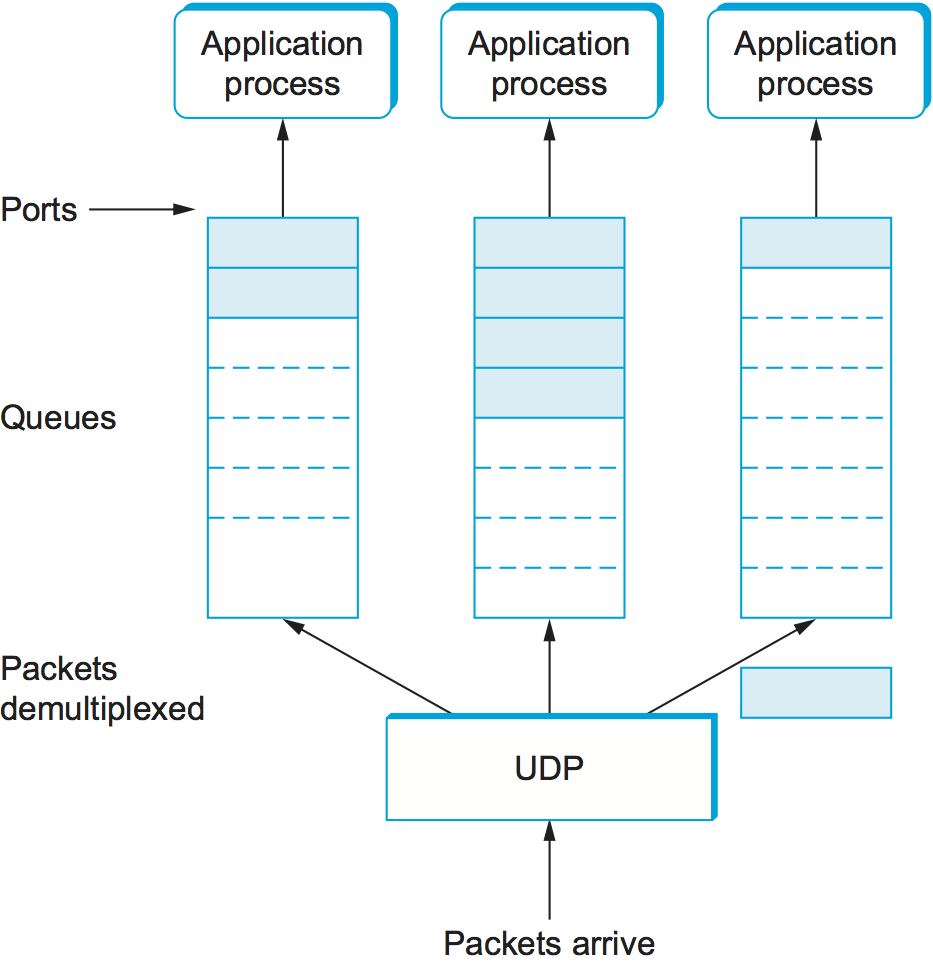
\includegraphics[width = 0.5\textwidth]{Pictures/UDP demultiplexing.png}
    \end{figure}
    \item \textbf{UDP checksum:} UDP does not provide any reordering, flow control but does provide a checksum optional in IPv4, but mandatory in IPv6. This checksum to make sure the correct port is being sent to. The checksum takes in input the source IP, destination IP, protocol number, and UDP length. This forms what is called the psuedo header,
\end{enumerate}

\section{TCP}
\subsection{End -To-End-Issues}
UDP was simple. Here are things make TCp harder.
\begin{enumerate}
    \item Need to start up and tear down the connection. since the resources need to be freed up.
    \item Variable RTT, so can not hard code delay time like ethernet stuff, which guarantees reception for 2500m long ethernet packets and all.
    \item out of order packets, as they travel in the internet. But we know packets defintely die out in 120 seconds, so we cna put this into a field called TTL, and take care of wandering packets. This can be changed by changing something called Maximum Segment Lifetime (MSL).
    \item We set up a connection depending on how much we can send, to fill up all our pipes. But what if the reciever can not handle that. We need a mechanism to learn the resources.
    \item network congestion (discussion later).
    \item TCP uses the sliding window algorithm on an end-to-end basis to provide reliable/ordered delivery. Another network only took care of hop to hop. That was bad since packets may not be delivered to intended place and extra work done by mid way nodes,. TCP packets only travel to network layer, but X.25 needed to travel to transport layer.
\end{enumerate}

\subsection{Segment Format}
\begin{enumerate}
    \item TCP is a byte-oriented protocol. Which means the sequcne numbers and acks are actually increments of bytes not packets.
    \item TCP’s demux key is given by the 4-tuple: (SrcPort, SrcIPAddr, DstPort, DstIPAddr)
    \item read actual segment from book. Copy paste stuff.
    \item Checksum field is used in exactly the same way as for UDP—it is computed over the TCP header, the TCP data, and the pseudoheader, which is made up of the source address, destination address, and length fields from the IP header.
\end{enumerate}

\subsection{Connection establishment and Termination}
\begin{figure}[H]
    \centering
    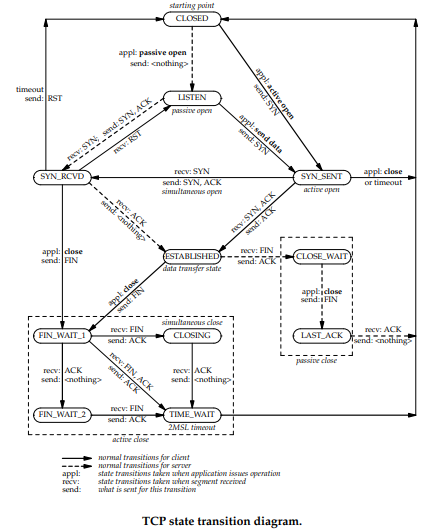
\includegraphics[width = \textwidth]{Pictures/TCP.png}
\end{figure}
Learn how to read this, and the three way handshake.

\subsection{Sliding Window Revisited}
\begin{enumerate}
    \item Need to know advertised window only.
    \item Once buffer starts filling up on receiving end, it starts to tell the sender, that I do not have x space left but x - unprocessed bytes I have, where x is the original space it has. This way the sender does not overwhelm the receiver. This is called Control Flow. The receiver then uses this advertised window to calculate the effective windwow.
    \item Once the receiver says I have no space, the sender starts Zero Frame Probes, these are frames of single byte of actual data that are sent on some time interval between 5 and 60s. This is used by the receiver to reply to the receiver, since the receiver never talks by itself.
    \begin{enumerate}
        \item Silly Window Syndrome- When a free window is advertised, does the sender jum in and send that much data or send the entire MSS (Maximum Segment Size). It needs to know when can it, or if ever can, since a smaller window size leads to it aggressivley filling up the pipe and not allowing bigger chunks to be sent, since the computer processes data segment wise, it would go byte by byte which can slow stuff down. Ususally the sender waits until it has one full MSS of free space. The question then comes how long should it wait? answered later.
    \end{enumerate}
    \item protecting against wrap around. Use time stamps. Need to learn this through examples, hard to explain in words.
    \item Keeping pipe full. with 16bits of sepeunce space we can only 64kb of data. How to resolve this? In TCP there is options called extended options. This allows a computer to shift the window size by an agreed amount to allow more sequence numbers.
\end{enumerate}

\subsection{To answer how to know when should I send data?}
\begin{enumerate}
    \item Nagle's: says wait till I have full MSS. Option of shutting it off, and allow SWS.
    \item Original: Running average of sorts with weighting to understand rate of change. Then calculate o a timeout as twice the calculated RTT.
    \item Karn/Patridge: modifies original, to not record RTT's during re-transmission. Original can take that into account and record a very small RTT the packet may simply be late. But also it just increases timeout by times two every time it needs to re transmit, exponential backoff.
    \item Jacobson/Karels:
    \begin{enumerate}
        \item Difference = SampleRTT - EstimatedRTT
        \item EstimatedRTT = EstimatedRTT + ( delta x Difference)
        \item Deviation = Deviation + delta (|Difference| - Deviation) where delta and delta are fractions between 0 and 1. That is, we calculate both the mean RTT and the variation in that mean.
        \item TCP then computes the timeout value as a function of both EstimatedRTT and Deviation as follows:
        \item TimeOut = mu x EstimatedRTT + phi x Deviation where based on experience, mu is typically set to 1 and phi is set to 4.
    \end{enumerate}
\end{enumerate}
\subsection{TCP extensions}
\begin{enumerate}
    \item Scaling Factor: increase the size of the window.
    \item Timestamp: TCP can read the actual system clock when it is about to send a segment, and put this time—think of it as a 32-bit timestamp—in the segment’s header. The receiver then echoes this timestamp back to the sender in its acknowledgment, and the sender subtracts this timestamp from the current time to measure the RTT.
    \item Timestamp: helps to figure when the packet got lsot and arrived too late. This will be discarded, buchecking with other timstamps of recent segments and seeing g this is too old and not in the current window.
    \item SACK: Selective ACK, since cumulative ACKS are generally used.
\end{enumerate}

\section{RTP}
Basically, it is a protocol bult on top of UDP, since the real time applications should not be tied down to what is provided, since packet losses may want to be treated differently, like in VOIP, just ignore packet loss since re-transmission is not fast enough.

\chapter{Chapter 6: Congestion Control}

\subsection{Queing Disciplines}
\begin{figure}[H]
    \centering
    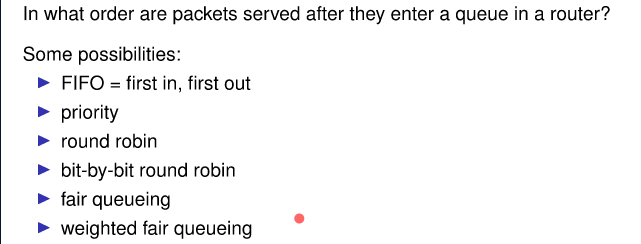
\includegraphics{Pictures/Queues.png}
    \caption{Types of Servicing: FIFO: self, Priority: Two different Queues, obvious problem of senders sending self priority}
    \label{fig:my_label}
\end{figure}
\begin{enumerate}
    \item FIFO:
    First in First Out, self explanatory. It is not very fair however. Whenever a person wants all the bandwidth they only need to send packets at higher rates. Can have priority, but hard to assign, priority is used for error messages, link updates however.
    \item Fair Queuing:
    Trying to share the bandwidth, using almost bit-wise round robin like spending with additional possible priority queue, or just priority set for every connection and the packets in those queues. Things like failure, or change in routes is most important.
    \begin{enumerate}
        \item Almost bit-wise, since packets are dealt according to size, and bits are not interleaved with one another. Also, this is used to decide which packets will be transmitted first, say, we have a long packet, and many short packets in another queue. The short packets will be scheduled first, then the long packets as the shorter packets take smaller time to send, but when the cumulative of shorter packets in one queue is longer, the longer packet instead will be sent. This way no one network is getting more service.
        \item Also note adding a smaller packet when transmitting a big packet does not stop the big packet transmission, in bit-wise round robin it would have been pre-empted.
    \end{enumerate}
    \item Weighted Fairness Queue, sort of like priorty to a certain queue.
    \item Fairness Index:
    \begin{figure}[H]
        \centering
        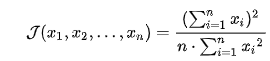
\includegraphics{Pictures/fairness index.png}
        \caption{Fairness index: $x_i$ is the bandwidth of $i^{th}$ connection}
        \label{fig:Fairness Index}
    \end{figure}
\end{enumerate}

\subsection{TCP Congestion Control}
\begin{enumerate}
    \item Additive Increase, Multiplicative Decrease: for every ack until start threshold add 1 or some agrred number to congestion window, after that add 1 or some agreed number for every RTT if there is any ack. If packet loss, by timeout or triple dup ack, multiply the current congestion window by 0.5 or some number between 0 and 1, and set start threshold to this value, changing congestion window to 1, restart start threshold.
    \item Fast Transmit, Fast Recovery:
    \begin{figure}[H]
        \centering
        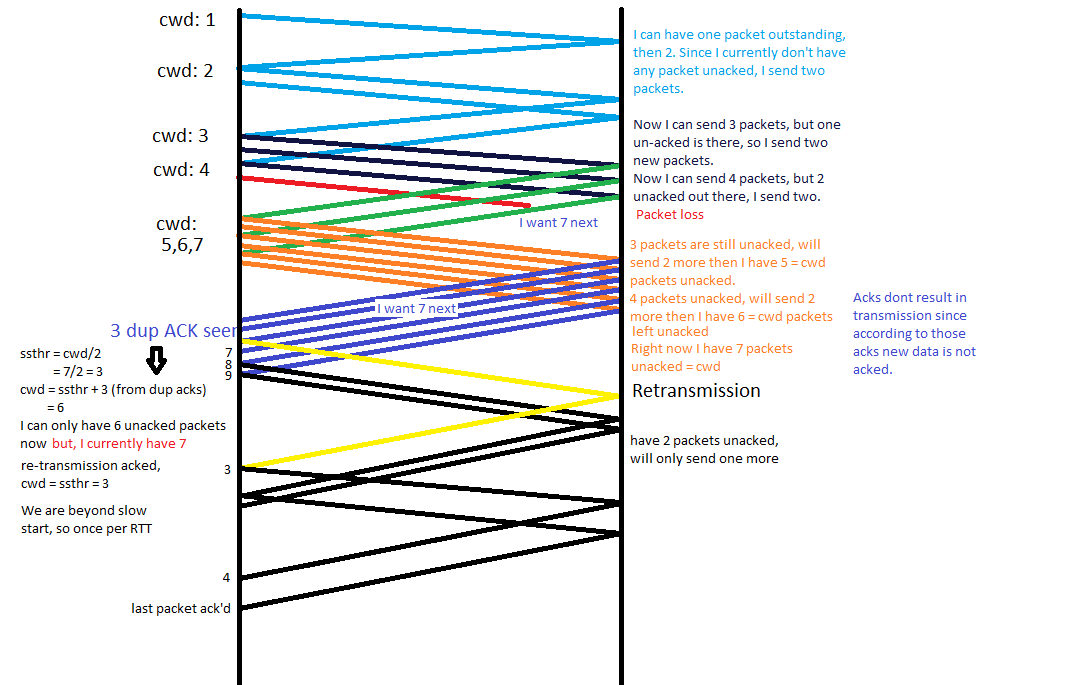
\includegraphics[width = \textwidth]{Pictures/fast transmit, fast recovery.png}
        \caption{FRFT}
        \label{fig:FRFT}
    \end{figure}
    \item TCP CUBIC: follow a cubic curve centered around last ssthr, this way I approach the ssthr carefully, but find the next ssthr quickly by exponential like growth.
\end{enumerate}

\subsection{Advanced Congestion Control}
\begin{enumerate}
    \item DECBit: This is an active Queue Management Algorithm, since action taken actively. router puts a bit into a header, which then is echoed by the peers acking the fact router queue is about to start droping some packets if the rate of sending packets is this high. A router sets this bit in a packet if its average queue length is greater than or equal to 1 at the time the packet arrives. This average queue length is measured over a time interval that spans the last busy+idle cycle, plus the current busy cycle. (The router is busy when it is transmitting and idle when it is not.)
    \item Random Early Detection: Router is starts dropping packet at a probability $p$, which increases as queue length reaches carrying capacity, in order to force the peers to have triple dup ack situation which automatically reduces traffic. Relies on peers employing TCP.
    \begin{enumerate}
    \item AvgLen = (1 - Weight) x AvgLen + Weight x SampleLen
        \item if AvgLen <= MinThreshold
        \begin{enumerate}
            \item queue the packet
        \end{enumerate}
    \item if MinThreshold < AvgLen < MaxThreshold
    \begin{enumerate}
        \item calculate probability P
        \item drop the arriving packet with probability P
    \end{enumerate}
    \item if MaxThreshold <= AvgLen
    \begin{enumerate}
        \item drop the arriving packet
    \end{enumerate}
    \end{enumerate}
    Time for AvgLen is taken every RTT, since actions are onyl reflected after that time.
    Higher the bandwidth of a link, it will provide more candidates for drops hence in that sense RED is pretty fair.
    \item Explicit Congestion Notification: ECT bit (ECN-Capable Transport). The other bit is set by routers along the end-to-end path when congestion is encountered, as computed by whatever AQM algorithm it is running. This is called the CE bit (Congestion Encountered).
    
    In addition to these two bits in the IP header (which are transport-agnostic), ECN also includes the addition of two optional flags to the TCP header. The first, ECE (ECN-Echo), communicates from the receiver to the sender that it has received a packet with the CE bit set. The second, CWR (Congestion Window Reduced) communicates from the sender to the receiver that it has reduced the congestion window.
    \item TCP Vegas: Use the sampled RTT bas base RTT to calculate expected and actual throughout, then depending on some thresholds increase, decrease the congestion window, or remain the same. This uses the idea that actual rate may be falling if congestion too much, and close to actual rate if congestion low. So if diff of actual and expected is close to 0 $\to$ congestion low, send more, and if diff too much $\to$ congestion too much, send less. The congestion window is increased/decreased linearly.
    
    Reaction to ECE bit should be same as actual packet loss.
\end{enumerate}

\subsection{Quality of Service}
Used for real time applications, where we need guarantee of service. In elastic applications delays are manageable, but for VOIP, etc. it is not. Real networks jitters and packets drops.

\begin{enumerate}
    \item IP and UDP are best effort protocol: \textbf{NO} guarantees about delivery or in time.
    \item TCP: solves mostly the delivery guarantee using transmissions, but not in time, only packets are eventually delivered. Goof for file transfer, file will arrive is guaranteed.
    \item TCP is not good enough for timely delivery due to jitters, hence appilcations protocol (RTP as before) is based on UDP. There is a delay distribution on the internet for packets, like a gamma distribution.
    \begin{figure}[H]
        \centering
        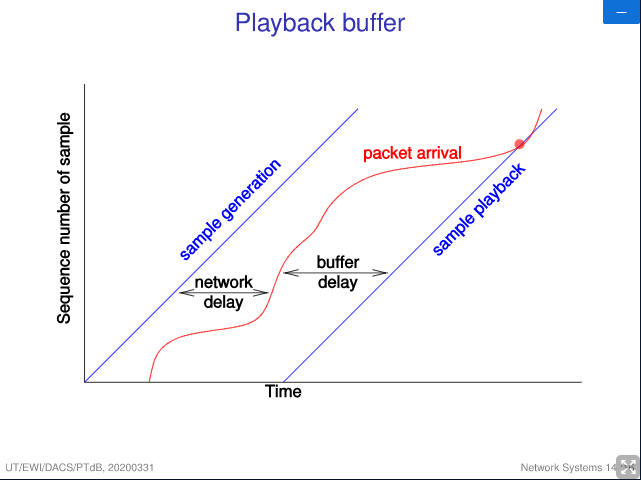
\includegraphics{Pictures/RTP QOS.png}
        \caption{So we can use a threshold like 90\% to say we shift the buffer playback by the time by which 90\% packets arrive, the rest will be thrown out. So all packets in between the two oblique lines, at left will be the earliest possible, and the right be the latest we can wait. We collect all the packets in between for generaitng the playback at that left line times.}
        \label{fig:my_label}
    \end{figure}
\end{enumerate}

Types of applications
\begin{enumerate}
    \item Elastic: File Transfers
    \item Real Time: VOIP
    \item Tolerant: VOIP
    \item Intolerant: Surgery Robots
    \item Adaptive: VOIP
    \item Non-Adaptive: THose who can't handle jitters
    \item Rate-Adaptive: VOIP $\to$ decrease quality
    \item Delay Adaptive: VOIP $\to$ tearing.
\end{enumerate}

Components needed to provide QOS:
\begin{enumerate}
    \item \textbf{Queing discipline}
    \item \textbf{Connection Treatment}: Priority.
    \item \textbf{Admission Control}:
    \begin{enumerate}
        \item Is it technically possible to provide QoS for both existing with new connection.
        \begin{enumerate}
            \item Need to know what connection \textbf{service} required.
            \item Need to know \textbf{traffic} characteristic of the new flow.
        \end{enumerate}
    \end{enumerate}
    \item \textbf{Policing}: Are the existing connections actuallly conforming to the traffic characteristic.
\end{enumerate}

\begin{enumerate}
    \item Traffic Specification:
    \begin{enumerate}
        \item This can be done using the concept of the leaky bucket analogy, r is rate of token filling, B is the bucket size, and R is the rate at which the router promises the provided rate. The rate at which service provided is at best B/R. The average rate is B/2R.
        \item \textit{It is only a model: it only describes how many packets a system may send when, but the system may use a different method to guarantee that it never transmits more than allowed by this model.}
    \end{enumerate}
\end{enumerate}

\subsection{IntServ, DiffServ}

\begin{figure}[H]
    \centering
    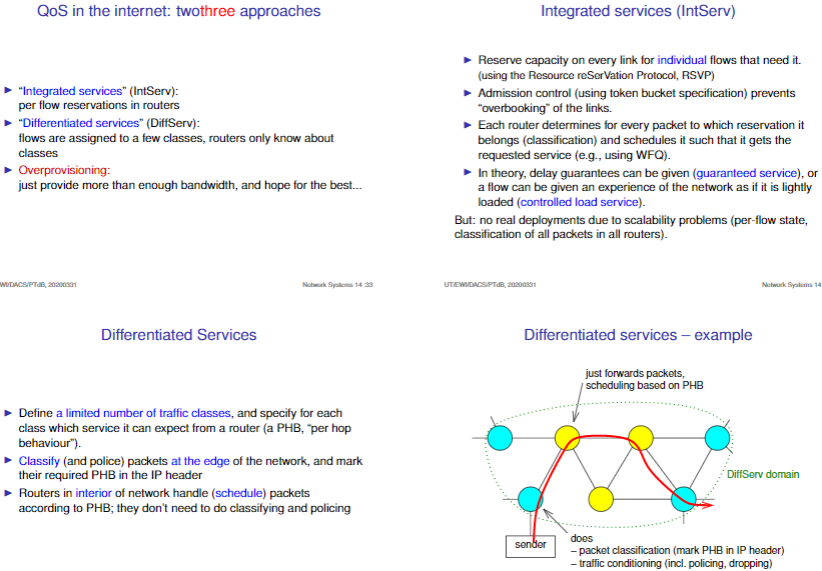
\includegraphics[width = \textwidth]{Pictures/IntServDiffServ.png}
\end{figure}

\begin{figure}[H]
    \centering
    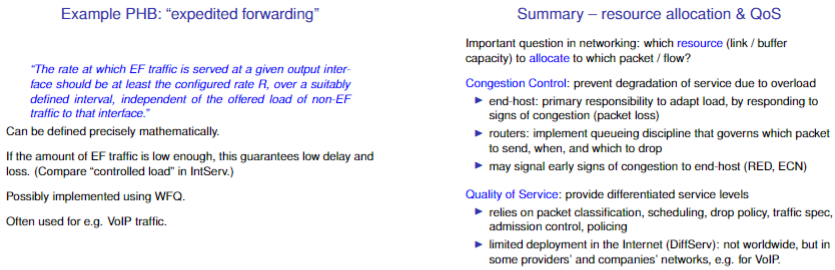
\includegraphics[width = \textwidth]{Pictures/IntServDiffServ2.png}
\end{figure}

\chapter{Chapter 7: End-to-End data}


\chapter{Chapter 8: Network Security}
http://www.unixwiz.net/techtips/iguide-ipsec.html

Encrypted using the private key of the sender. So if wrong, then not accepted, if yes considering a trust, we get the data.

WEP- IV, too small, communicated in plain text. Easy to brute force if enough data.

WPA- Authentication Server(Radius), get key from AP

SSH tunnelling only works if you have a device behind the firewall.


(A,0,-) always in Djikstra

ARP is on the user computer.

SeqNum for Link State packets

Unless FIN received remote sender can still send data even if I sent FIN.

WFQ needs Shecduler to be installed too.

Link State packets have sequence numbers if the same sequence number is seen they do not forward it.

Learning Bridges use spanning tree algorithm, so no loops, the packet reaches only the end host.

cwnd += $mss^2$/cwnd
only if ACK is mss, not a smaller byte, Instead use the formula 
cwnd += mss(n/cwnd) where n is the number of byte ackd in each ack.

-Bridges store all MAC for every computer (40 from that question)
-Routers store the range for every LAN, (4 in that question) given route aggregation not possible.
- ARP of every computer stores the MAC of every computer on the LAN and all the routers the LAN is connected to. (9+2 = 11 in that question).

The actual window size will be 280*16 = 4480 bytes, and thus include all sequence numbers up to 4599. Which comes from effective window being 120bytes. So if we say window scaling is used, and scale $2^4$ = 16 * advertised window, we mean we have space for 280*16 bytes.

Careful with the dvr, difference between getting to know in that update and sending in the same update.

fast transmit at smaller windows and more retransmissions due to re-ordering.

PAWS is WS not used for short fat pipes, large bandwidth and small RTT. wraparound propotional to bandwidth not RTT. On small RTT no window scaling needed but wrap around possible.

window scaling fulfills lack of bits in window header.

ECN reduces packet loss, by telling people of congestion.
start 50 / 50 when FQ (not WFQ). then fulfill smaller one and rest for larger one.

Allow packets destination port >= 1024 or use Statefull Firewall.
Webcam can be hacked using TCP/IP header, basically if device and is connected to net, we can use firewall to block it.

When pakets are tunneled they get added header bytes, hence more fragmentation therefore MTU is smaller for IPv6 tunneled as IPv4, since less data more header.

LS does not have count to infinity problem period.
PIM-SM do not who sender intitially so everyone joins a designated shared tree then connected to sender if there is one.

sending FIN incrementns ACK that is sent.

\begin{table}[H]
    \centering
    \begin{tabular}{|c|c|c|}
    \hline
         WS & PAWS & use \\ \hline
         0 & 0 & short slim \\ \hline
         0 & 1 & short fat \\ \hline
         1 & 0 & long slim \\ \hline
         1 & 1 & long fat \\ \hline
    \end{tabular}
    \caption{Caption}
    \label{tab:my_label}
\end{table}

for the TCP Vegas question, make a line equation between those which have delay. The queuing delay only occurs between them as. Then the gradient is the link speed. By extrapolating to the point where delay is 0, that will give you how many packets are not in queue, so 20-5 = packets in queue.

Difference between updates made and number of iterations done.
Large bandwidth delay means convergence to best cwnd is slow.
If additive increase parameter increased but not for others, then higher throughput, but not starving.

When senders increased, token not necessarily increased.
If total 20 + 70 = 90 < 100. Then 10\% idle already implied no need to take ratio.

sometimes only split horizon, and not poison reverse.

**RQRQRQRQRQRQRQRQRQRQRQRQRQRQRQRQRQRQRQ**


\chapter{Chapter 9: Applications}

HTTP vers:
1.0, 1.1

1.0 and 1.0 with parallel connections
1.0 does not have connection persistence,
Handshake made, request forwarded, session closed.

1.1 and 1.1 with pipelining.
while 1.1 has persistent connections.
handshake made, request forwarded, session stays active.

\end{document}